\documentclass{book}
\usepackage{graphicx}
\usepackage{url}
\usepackage{csquotes}
\usepackage{textcomp}
\usepackage{menukeys}
\usepackage[hang,flushmargin]{footmisc} 
\graphicspath{ {images/} }
% listings package and parameters provide formatting for
% source code examples
\usepackage{listings}
\usepackage{color}
\definecolor{dkgreen}{rgb}{0,0.6,0}
\definecolor{gray}{rgb}{0.5,0.5,0.5}
\definecolor{mauve}{rgb}{0.58,0,0.82}
\lstset{frame=tb,
	language=Python,
	aboveskip=3mm,
	belowskip=3mm,
	showstringspaces=false,
	columns=flexible,
	basicstyle={\small\ttfamily},
	numbers=left,
	numberstyle=\tiny\color{black},
	keywordstyle=\color{black},
	commentstyle=\color{gray},
	stringstyle=\color{black},
	breaklines=true,
	breakatwhitespace=true,
	tabsize=3
}
\begin{document}
\frontmatter
\pagestyle{plain}
\begin{titlepage}
	\title {\huge \textbf{Introduction to Data Analysis for Accountants: A Python Approach}}
	\date{}
	\author{Stephen Perreault, PhD, CPA}
	\maketitle
\end{titlepage}
% copyright page
\begingroup
	\parindent 0pt
	\parskip \baselineskip 
	\textcopyright{} 2017 Stephen J. Perreault 
	
	\begin {center}
	
\includegraphics  [scale=1.5]{creative_commons_license}
	\end {center}
	
	This work is licensed under the Creative Commons Attribution-NonCommercial-NoDerivatives 4.0 International License. To view a copy of this license, visit http://creativecommons.org/licenses/by-nc-nd/4.0/ or send a letter to Creative Commons, PO Box 1866, Mountain View, CA 94042, USA.
	
	Version 0.1.0: August 2017
\endgroup
\tableofcontents

% acknowlegments
\begin {center}
\newpage
\textit{
To Kathleen, Lyla, Willy, and Matilda.}
\end {center}

\mainmatter	
\parindent 0pt
\parskip \baselineskip 

% Chapter 1
\chapter{Introduction}
\section{What is data analytics?}
\section{Who is this book for?}
\section{Hardware and software requirements}

Assumes you are using a Windows-based PC. Mac versions in the future.

% Chapter 2

\chapter{Version control}
\section{Why you should care about version control}

Imagine that the audit engagement team which you have been assigned to is in need of a tool that can assess the valuation of an audit client's stock options using the Black-Scholes-Merton valuation model.\footnote{It's not important to understand what the Black-Scholes-Merton model is to appreciate this example. However, if you're curious, BSM can be used, among other things, to determine the price of certain types of stock options.} The tool needs to be simple to use, scalable, and compatible with a wide variety of operating systems. Knowing your reputation as a skilled programmer who works well under pressure, your supervisor has given you 24 hours to write the Python module to perform this assessment.

You spend the night hunched over your keyboard working frantically to complete the assigned task before the deadline. Your source code undergoes numerous changes as you squash bugs, improve performance, and add extra features that you believe the engagement team might find useful. As the sun begins to rise the next morning, you realize that you have successfully completed the task. You have developed a functional software tool that you are sure will impress your supervisor. 

Before emailing the Python script to the engagement team, you decide to make some minor tweaks to your code in order to slightly improve the tool's performance. After making the seemingly harmless modification to your code, you test the script one final time and are horrified to discover that the change you made has caused an error which has rendered the program non-functional.

Frantically, you scan through the script, hoping to identify the changes that you made which might have caused the program to break. You haphazardly remove a few lines of code that you think may be the culprit but that doesn't seem to do the trick - the program still crashes. In addition, this deletion causes another portion of the program to break. Feeling hopelessly lost, you begin to realize that you may be forced to start the project from scratch. What will you possibly tell your supervisor?

As the example above has hopefully demonstrated, it is incredibly important for programmers to keep track of the changes made to their source code over time. This process can seem daunting, especially for large projects with many different developers working on the code base simultaneously. Fortunately, modern developers can rely on version control systems to help manage these changes. If an error is introduced into the code, the developer can simply turn back the clock and revert to an earlier stable version. 

Since we're going to be writing a significant amount of computer code as we work our way through this book, it makes sense to start by learning a bit about how version control works. In this chapter we will learn how to use version control to track changes to our individual projects. We will also learn how to create an online repository of our source code which can be shared with others and used as an online software development portfolio.

\section{Introducing Git}

In this book we will be using the widely used and popular version control system Git\texttrademark. Git was created in 2005 by Linus Torvalds, the famous creator of the popular operating system Linux. In addition to providing developers with a history of all the individual changes that have been made to their projects, Git can also be used to track changes for developers working collaboratively. 

As an example, let's say that you and a coworker have been assigned the task of writing a piece of software and will both need access to the source code during development. To facilitate this, you could post the code on a shared network drive or a file hosting service that you and your coworker can access. This method would probably work just fine unless the two of you are working on the same code file at the same time. If that happens, one of you would have your work overwritten and erased. Git can keep that from happening. If you and your coworker are both making changes to the same source code file, Git will save two copies. Later on, the changes can be merged together without losing any of the earlier work. 

Unfortunately, Git has an reputation as being difficult for beginners to use (which is undeserved in my humble opinion). This mostly stems from the fact that it does not have a graphical user interface; rather, users access the features of Git by typing in commands using the system terminal or command line. While there are GUI tools available for Git, working from the command line is an important skill set for an aspiring Python programmer to develop. As a result, we will be using the command line when working with Git in this book. 

\section{Introducing GitHub}

While Git is handy version control system for working with projects locally on our computers, there are often times when we want to share our projects with others. To do this, we'll be using the online service GitHub\texttrademark. GitHub is basically an online social media service; however, the primary type of information being shared on GitHub is source code as opposed to cat pictures!\footnote{This attempt at humor is actually not factually correct - projects posted on GitHub can contain images if the user wishes.} Throughout this book, we'll be using GitHub and Git in tandem in order to manage changes and share our projects with others.

\begin{figure}[h]
	\caption{Registering for a GitHub account}
	\centering\includegraphics[width=.90\textwidth]{/Chapter2/Figure_1}
\end{figure}

Although desktop clients are available, GitHub can be used without installing any software onto our computers. You simply have to sign up for a free GitHub account. Let's go ahead and do that now by visiting \texttt{https://github.com}. The sign up process is as easy as registering for any other social network. Note that you'll want to sign up for the free plan. GitHub also offers paid subscriptions with more advanced features; however, these features our unnecessary for the purposes of this book.

I encourage you to personalize your GitHub profile by uploading a recent picture of yourself. You may also wish to include  other relevant background information  or links to a webpage (if you have one). However, remember that the information which you include in your profile is publicly viewable - only provide information you would be comfortable sharing with others, including future employers. Once you're finished, let's move on to installing Git.

\section{Installing Git}

If you are using a computer that is connected to a campus network (such as a machine in an on-campus computer lab), there is a good chance that Git is already installed.\footnote{If you see an entry for ``Git Bash" somewhere on the computer's Windows Start Menu, then Git is already installed.} However, if you plan on working through this book using your personal computer (which is probably the case) you will need to install Git on that device.

You can find the installation package on Git's homepage which is located at \texttt{https://git-scm.com/downloads}. Download the Windows release and then open the executable. Accept all default installation settings by clicking "Next" until the installer begins extracting the program files to your hard drive. Once the installation is complete, you should be able to find a folder called ``Git" within the Windows start menu. Inside the folder you should see a shortcut to a program called ``Git Bash." Clicking this shortcut will launch the Git command line. Let's go ahead and do that now.

\begin{figure}[h]
	\caption{The Git homepage showing the link to the installation package}
	\centering\includegraphics[width=1\textwidth]{/Chapter2/Figure_2}
\end{figure}

Launching ``Git Bash'' for the first time will display an empty terminal window which should look a bit like Figure 2.2. The first line of output in the terminal should contain your Windows account name as well the hostname of the computer you are using (we will be ignoring this information). The dollar sign (\$) represents the terminal prompt which is where we will be typing all of our Git commands.

\begin{figure}[h]
	\caption{An empty Git Bash terminal}
	\centering\includegraphics[width=.90\textwidth]{/Chapter2/Figure_3}
\end{figure}

With the terminal open, let's go ahead and tell Git who we are. Type in the following command:\\ \\ \texttt{git config -- global user.name "My Name"}

Obviously, you'll need to replace the words in quotation marks with your own name! You can use your full name, a nickname, or a handle that you regularly use online. Git will attribute any changes you make to projects to the name that you provide here. You'll also need to provide Git with your email address (make sure it's the same email address you used when signing up for GitHub) using the following command: \\ \\ \texttt{git config --global user.email "my\_email@my\_email.com"}

\section{Creating your first repository}

Both GitHub and Git store individual projects in ``repositories" (often referred to as ``repos" for short). Any files that make up your projects (e.g., source code, image files, text files, etc.) can be stored inside a repository. Let's go ahead and create a repository right now. 

Log into your GitHub account and click the ``Create New" button (this looks like a small + sign to the left of your profile picture at the top of the webpage). Select the option to create a new repository. Name this new repository \texttt{my\_first\_repo} and leave the ``Initialize this repository with a README" box unchecked (your screen should look similar to Figure 2.4). You can also give the repository a brief description if you like. Once finished, click the ``Create repository" button. 

\begin{figure}[h]
	\caption{Creating a new repository using GitHub}
	\centering\includegraphics[width=.90\textwidth]{/Chapter2/Figure_4}
\end{figure}

You've now created a repository for your project on GitHub. However, the majority of the work you do on your projects is likely going to be performed on a local computer instead of online (for example, we want to be able to work on our projects in places where we don't have an internet connection). Therefore, we are also going to create a local repository for our project using Git. We'll link the local Git and online Github repos together later in the chapter.

Before you create a new local repository, you're going to need to create a location on your hard drive (or network drive if you're using a lab computer) where that repo will live. Re-open the Git Bash terminal and enter the command: \\ \\ \texttt{mkdir \textasciitilde/my\_first\_repository}
 
This will create a directory (or folder) called \texttt{my\_first\_repository} where your repository and its related files will be stored on the drive.\footnote{This folder will be created off of the top level directory on the drive. For most Windows users, this will be \texttt{C:\textbackslash users\textbackslash your\_user\_name}. However, it may also be the top level of the network drive if you are using a PC in a campus computer lab (e.g., \texttt{G:\textbackslash}). You can find the location of the top level directory by using the \texttt{\textasciitilde/} command.}

Now navigate to the new directory you just created using the command:

\texttt{cd my\_first\_repository}

As you may have guessed, \texttt{cd} stands for ``change directory.'' Note that if you want to navigate out of this directory and back to the top-level directory, simply use the command:

\texttt{cd}

Notice that the path displayed above the command prompt changes depending on the directory you are currently located in. This is demonstrated in Figure 2.5 (note that my top-level folder in this example is G:\textbackslash).

\begin{figure}[h]
	\caption{Navigating directories using Git Bash}
	\centering\includegraphics[width=.90\textwidth]{/Chapter2/Figure_5}
\end{figure}

Let's navigate back to the \texttt{my\_first\_repository} directory. We're now going to initialize a new Git repository in this directory by using the command:{\footnote {You can tell that this is a command which is specific to Git (as opposed to a system command such as \texttt{mkdir} or \texttt{cd}) due to the fact that is prefixed by the term \texttt{git}.}} 

\texttt{git init}

If successful, Git will tell us that it has initialized an empty repository in the filepath we have chosen. Congratulations - you have created your first Git repo!

\section{Adding files to your repository}
Now that we have created a working repository, it is time to begin adding files. Every Git repository you create should contain a file that provides a brief written overview of the project. We'll be adding a file called \texttt{README.md} to our repository which contains this information.\footnote{See \texttt{https://gist.github.com/jxson/1784669} for an excellent template for creating informative project README files.}

This \texttt{README.md} file must be created as a simple text file (which means that the file contains no data other than text). We can create such a file using any text editing tool. Since all copies of Windows come with the ``Notepad'' text editor, this is the program we will be using to create our \texttt{README.md} file. Find the Notepad program on your computer and open it (a shortcut to the program can typically be found in the Accessories folder within the Windows Start Menu).

Once Notepad has been opened, type the name of your project on the first line of the file (this is usually the same name as your repo name). Inserting the hash character (\#) prior to the project name will make this text slightly larger than the remaining text in the file. (It is good practice to prefix all section headings in your \texttt{README.md} files with \#). On a separate line of the file, provide a brief description of the project. Note that, in practice \texttt{README.md} should contain far more information than this; however, this level of description is sufficient for our current purposes. Figure 2.6 provides an example of what this file might look like.

\begin{figure}[h]
	\caption{\texttt{README.md} for the project}
	\centering\includegraphics[width=.90\textwidth]{/Chapter2/Figure_6}
\end{figure}

\begin{figure}[h]
	\caption{Saving to the repository directory}
	\centering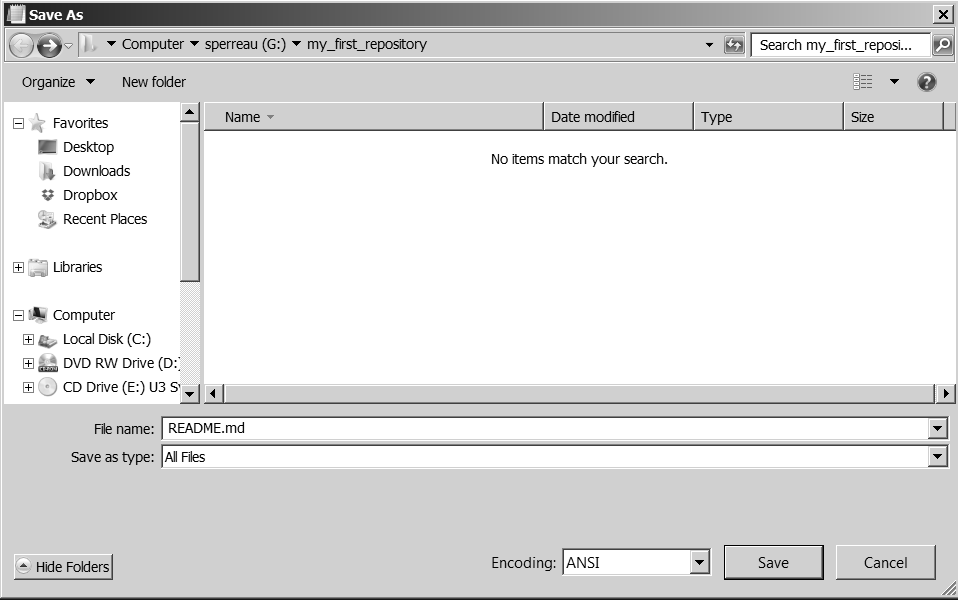
\includegraphics[width=.90\textwidth]{/Chapter2/Figure_7}
\end{figure}

When your text file looks sufficient, it's time to save it to the directory that we created our repository in. In Notepad, click ``Save as" from the ``File" dropdown menu. Then navigate to the repository directory. Type \texttt{README.md} as the ``File Name'' and click the ``Save'' button. See Figure 2.7.

We have now saved the file to the directory where we created our repository; however, we now need to specifically tell Git to add the file to our repo and begin tracking it. To do this, we'll need to re-open the Git Bash terminal. 

If necessary, navigate back to the directory where the project repository is located. Then enter the following command:

\texttt{git add README.md}

Now that the file has been added to the repository, let's check the status of the repo using the command:

\texttt{git status}

The output should look something like the output in Figure 2.8. 

\begin{figure}[h]
	\caption{Checking the repository status}
	\centering\includegraphics[width=.90\textwidth]{/Chapter2/Figure_8}
\end{figure}

Let's take some time to review this output. First, notice that Git has indicated that this repository is the ``(master)'' branch of the repository. We haven't yet created any additional branches for this project so this is to be expected. We'll talk more about incorporating multiple project branches later in the chapter.

The next line of Git output tells us that we are currently creating the ``initial" (or first)  commit for the repository. Whenever we save changes to a repository, we refer to this as ``commiting the changes" in Git parlance. Commits also provide us with a snapshot of our project at a particular point in time, allowing us to restore the project to one of these previous states if so desired. The output indicates this initial commit will involve adding a new file to the repository called \texttt{README.md}, as expected. Note that we should always check the status of our repository using \texttt{git status} prior to commiting any changes.

Since the status of our repo looks as expected, let's go ahead and commit the change. This can be done with the command:

\texttt{git commit -m "Add README.md"}

The ``commit" command tells Git to commit all pending changes to the repository. We have also included the \texttt{-m} flag to associate this commit with a brief message indicating what changes are being recorded to the repository. You should always include such messages when executing a commit so you have a record of the changes made to your project over time. You can verify that your commit worked by checking the status of the repo again using \texttt{git status}. You will notice that there are no other changes scheduled to be commited.

\section{Pushing commits to GitHub}
So far we have only modified the version of the repository that is stored locally on our individual computers. However, at some point we will likely want to share our repo online with others. We can do this by linking our Git repository to our GitHub account and ``pushing" the changes to the GitHub repository that we created earlier. Let's do this now.

We first need to tell Git that a remote (or online) version of our repository exists. We do this by providing Git with the web address (url) for our GitHub repository. The format for this address is:

\texttt{https://github.com/user\_name/repo\_name}

where \texttt{user\_name} and \texttt{project\_name} are replaced with your GitHub username and the name of your GitHub repository.

We'll point Git to this GitHub repository using the following command:

\texttt{git remote add origin https://github.com\_name/repo\_name}

The command tells Git that our project files can now be sent to a remote location (called ``origin") which can be found at the github address provided. We can verify that we have configured our repository correctly be using the following command:

\texttt{git remote -v}

The \texttt{-v} flag tells Git to provide a verbose description of the repository which contains the url name. If your repository is set up correctly, the output will look similar to Figure 2.9.

\begin{figure}[h]
	\caption{Checking the remote origins for a repository}
	\centering\includegraphics[width=.90\textwidth]{/Chapter2/Figure_9}
\end{figure}

Note that the origin connection is listed twice with the descriptors \texttt{(fetch)} and \texttt{(push)}. This means that we are both able to \textit{push} changes to and \textit{fetch} changes from the online GitHub repo.

Now that we've verified that our connections are configured appropriately, we can actually push our changes up to the GitHub remote. The following command tells GitHub to push the master branch of the repo (the only branch we have created so far) to the origin connection we just established. Note that you may be prompted to login to GitHub again when issuing this command.

\texttt{git push origin master}

You can verify that the push command worked successfully by visiting the GitHub repo page using your web browser. You should see that the file \texttt{README.md} has been added to the online repository and that the repo description has been appropriately updated based upon the contents of the file.

\begin{figure}[h]
	\caption{Verifying the push command on GitHub.com}
	\centering\includegraphics[width=.90\textwidth]{/Chapter2/Figure_10}
\end{figure}

\section{Reverting a commit}
Since we've only pushed one commit to the example repository we've been working with in this chapter, let's go ahead and push another one now. Open Git Bash and enter the following command from within the repository directory:

\texttt{touch badfile.bad}

\texttt{Touch} is a terminal command that creates an empty file. For this example, we simply want to make a change to the repository that we can commit. Adding a new file using the \texttt{touch} fulfills that objective nicely.

You can see the contents of the working directory by using the terminal command \texttt{ls}. Entering this command should display the following files which currently make up the repo directory: \texttt{README.md badfile.bad}.

Now, using the methods discussed in the previous two sections, perform the following steps:

\begin{itemize}
	\item Add \texttt{badfile.bad} to the local repository
	\item Check the local repository status, making sure that \texttt{badfile.bad} is marked as an addition to be commited
	\item Commit the change to the local repository with the message \texttt{"Add badfile.bad"}
	\item Push the new commit to the remote version of the repository on GitHub
\end{itemize}

Note that the GitHub remote origin connection that we established earlier is permanently associated with the repository unless we manually remove it (you can verify this with \texttt{git remote -v}). So you do not have to re-establish this connection every time you push commits for this repo to GitHub.

If you have completed these steps correctly, when you visit the repository page on GitHub.com you will see that \texttt{badfile.bad} has been added to the online repo. In addition, GitHub now tells us that two commits have been processed to this repository, as visibile in Figure 2.11.

\begin{figure}[h]
	\caption{Displaying the list of commits for a GitHub repository}
	\centering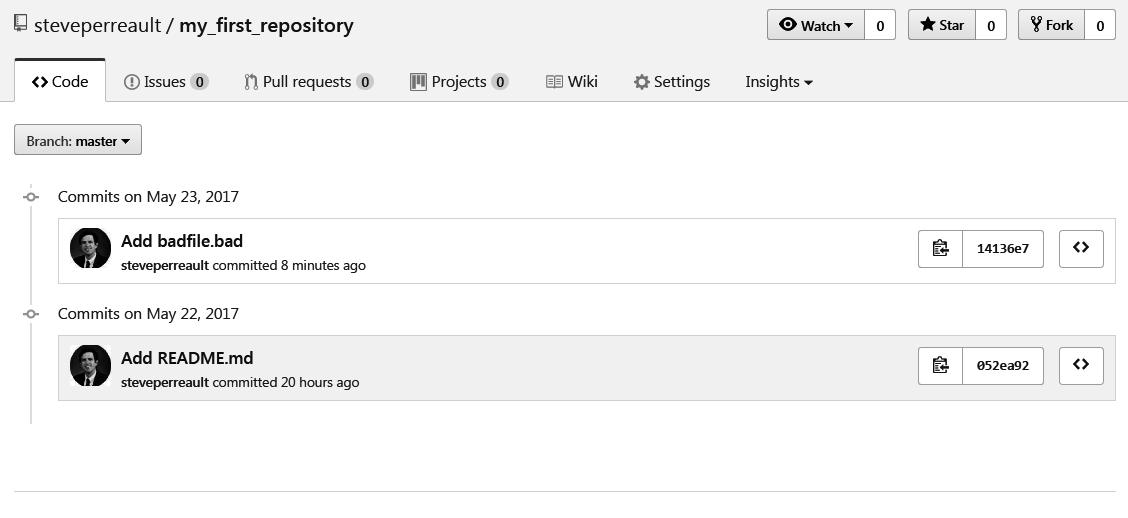
\includegraphics[width=.95\textwidth]{/Chapter2/Figure_11}
\end{figure}

There may be times when we push a commit that changes a branch in some undesirable way. For example, let's assume that the last commmit pushed to GitHub was in error and that we \textit{really} don't want \texttt{badfile.bad} to be including within the \texttt{my\_first\_repository} repo. In this instance, we may want to revert the repository back to what it looked like before we made the commit. We can do this using Git's \texttt{revert} command. We'll first revert the local repository to the earlier state using Git Bash and then we will push the modification of the local repo to GitHub.

To start, obtain a listing of all of the changes made to our local repository by using the command: \texttt{git log}.\footnote{Using the Git command \texttt{git log --oneline} will display each commit on single line. This may be useful for repositories with large numbers of commits. Also, your terminal may make your log scrollable if the output exceeds the height of its window. In this case, you can use your keyboard's arrow keys to scroll through the log. Entering \texttt{q} will return you to the terminal prompt.} For example, as seen in Figure 2.12, the log file for the  \texttt{my\_first\_repository} repo currently lists two commits (Git displays the most recent commits first). In this example, we want to revert our repo back to the state that existed immediately after the first commit where \texttt{README.md} was added. In order to maintain an accurate change history, Git treats the reversion as an additional commit.

\begin{figure}[h]
	\caption{Displaying the log file for a local repository}
	\centering\includegraphics[width=.95\textwidth]{/Chapter2/Figure_12}
\end{figure}
 
 To do this, we'll use the following Git command:
 
 \texttt {git revert 14136e7 --no-edit}
 
 where ``14136e7" refers to the first seven digits of the identifier for commit we want to revert (Git does not require us to type the full identifier number).\footnote{Note that the identifier number you type here will be unique to your specific repository.} The \texttt{--no-edit} flag associates a default description with the reversion commit, which is sufficient for our purposes. Once the command has been entered, displaying the log file for the repository using \texttt{git log} should now show the reversion commit as the most recent entry.
 
 Now all that's left to do is to push this latest commit to GitHub using \texttt{git push origin master}. Once this has been done you will have successfully reverted the commit!

\section{Cloning a repository}
In addition to being able to ``push" a project of your own to GitHub, you can also use Git grab a copy of a repository that another GitHub user has created. This is done using Git's \texttt{clone} command.

To clone an existing repository, open Git Bash and enter the following command:

\texttt{git clone https://github/user\_name/repository\_name}

where \texttt{user\_name} and \texttt{repository\_name} represent the repository name and GitHub username associated with the repository to be cloned. Note that the \texttt{clone} command will do the following:

\begin{itemize}
	\item Create a new local folder that has the same name as the repository being cloned
	\item Initialize the new folder as a repository using \texttt{git init}
	\item Copy all of the cloned repository's files and commits to the new local folder
	\item Create a remote connection named \texttt{origin} which points to the URL where the repository was cloned from
\end{itemize}

Pay careful attention to that last bullet point. Unless you change the default remote origin connection created by \texttt{clone}, any commits you push to GitHub will be recorded to the GitHub repository that was originally cloned (the owner of the repository will need to approve the changes). 

If you want to push changes made to your locally cloned repository to \textit{your own} GitHub account (as will usually be the case), you can use the following command:

\texttt{git remote set-url origin https://github.com/user\_name/repository\_name}

where the web address reflects the URL of the GitHub repository that you want to push changes to (this will typically be an empty repository you have created in GitHub following the steps discussed earlier in the chapter).

\section{Advanced: Creating branches}
When a repository is initially created, by default it contains a single branch called the ``Master'' branch. This master branch is considered the definitive branch of the project. As such, with larger projects, changes to the master branch should be considered carefully.

However, it is possible for a repository to contain other branches which are not considered separate from the master branch. At the time of their creation, these branches contain a perfect copy of the contents of the master branch. However, because they are only a copy of the master, developers can make edits and changes to the new branch worrying about corrupting the master branch. In this way, your master branch can be insulated from inadvertent errors introduced by changes made in other branches. Ultimately, commits made in these other branches can be merged into the master branch once the changes are determined to be stable.

Let's create a new branch of the /texttt{my\_first\_repository} repository that we created earlier in the chapter. From the local directory for the repository, enter the command:

\texttt{git branch bugfix1}

where \texttt{bugfix1} represents the customizable name for the new branch.\footnote{Note that software development teams often create branches to manage specific project issues, so branch names such as \texttt{bugfix1} are somewhat common.} To switch from the master branch to the new branch you just created, use the command:

\texttt{git checkout bugfix1}

Now push this new branch to GitHub using the command we learned earlier:

\texttt{git push origin bugfix1} 

You can now verify that the separate branches have been pushed to GitHub, as demonstrated in Figure 2.13. Note that the commit history for the \texttt{bugfix1} branch also inherited any commits that were made to the master branch at the time that the \texttt{bugfix1} branch was created. However, going forward, any changes made to the master branch or the \texttt{bugfix1} branch will be tracked separately until the two branches are merged (as discussed in the next section).

\begin{figure}[h]
	\caption{Viewing branches in GitHub}
	\centering\includegraphics[width=.95\textwidth]{/Chapter2/Figure_13}
\end{figure}

We can now switch back and forth between the two branches using \texttt{git checkout} from within the terminal. We can switch between the branches in the remote repository hosted on GitHub as well. Note, however, that since our repository now contains two branches, we will need to be careful to ensure that we are working off of the \texttt{bugfix1} branch until we are ready to merge our changes into the master branch. In addition, we will need to remember to provide the appropriate branch name when pushing commits to GitHub.

It may be helpful to recall that we can use the \texttt{git status} command we discussed earlier to identify which branch is currently active within the terminal. Additionally, the command \texttt{ git branch -r} can be used to obtain a list of all remote branches for a repository.

\section{Advanced: Merging branches}

Let's see you've finished work on the \texttt{bugfix1} branch and now want to merge the changes into the master branch. To do this, switch to the branch you wish to merge into using \texttt{git checkout} (in this case, you would switch to the master branch) and enter the following command:

\texttt{git merge bugfix1}

We can then push the changes to the master branch of the remote repository on GitHub using:

\texttt{ git push origin master}

Note that if we view the commit history for the master repository on GitHub (or locally by using \texttt{git log} within the termimal), we will that the changes made to the repository as a result of the merge are listed as a separate commit. This makes it easy to revert a merge if we so wish (we would simply follow the steps for reverting a commit discussed earlier).

For purposes of working through the exercises in this book, you should never record changes (commits) to multiple branches of a project concurrently. Doing so can cause conflicts when merging the two branches together. For example, let's say a user changes the same line of code differently within two branches that they are attempting to merge together. In this case, Git will not be able to complete the merge cleanly because it doesn't know which change is the ``correct" one to be retained. Git contains a number of features that knowledgeable users can employ in order to reconcile conflicts; however, these tools are beyond the scope of this text.

\section{Summary}
This chapter discussed the reason for using a version control system when developing your software projects. It introduced the Git package for local version control and the GitHub platform for sharing project code remotely. The concept of project repositories (repos) was introduced and the process for adding files to and making changes to repositories (commits) was discussed. The chapter described how local repositories can be stored on and retrieved from the GitHub platform. Finally, basic concepts relating to branching and merging were introduced.

Note that this chapter merely scratches the surface of what you can accomplish using Git. If you are interested in learning more about how you can use Git and GitHub in your software development projects, a good starting point would be the respective documentation for the two tools. This can be found at:

\begin{itemize}
	\item Git: \texttt{https://git-scm.com/documentation}
	\item GitHub: \texttt{https://guides.github.com}
\end{itemize}

\section{Exercises}
\begin{enumerate}
	\item What is the purpose of a version control system such as Git? Mention three benefits of using such a system.
	\item Why might a developer choose to also use a social media platform such as GitHub instead of just using the Git version control system locally?
	\item Conduct some brief internet research to identify competing websites that offer services similar to GitHub. Do any such sites exist?
	\item How can the concept of branching prevent unintended problems from occurring during the software development process?
	\item Create a local repository using Git. Name the repository \texttt{my\_fav\_picture}. This repository should contain:
	\begin{itemize}
		\item a README.md file which contains the name of the project and a brief description of the project. 
		\item a humorous image which you found online 
	\end{itemize}
		When finished, push the repository to your personal GitHub account.
	\item The \texttt{Ch2\_Ex2} repository located on this book's GitHub page contains a single file which includes the the text of my favorite poem. Clone a copy of this repository to your local drive and then:
	\begin{itemize}
		\item Revert the most recent commit that was made to the repo
		\item Modify the contents of \texttt{favorite\_poem.txt} so it contains the text of \textit{your} favorite poem.
	\end{itemize}
	When finished, push the modified repo to \textit {your own} GitHub account. (Note that you will need to change the URL that the origin remote connection points to in order to push to your own account!)
	\item Create a new local branch for the repository that you created in the first exercise. Then:
	\begin {itemize}
		\item Add an empty file called \texttt{addition.txt} to the new branch and commit the change.
		\item Merge the new branch into your master branch
	\end {itemize}
	When finished, push the completed project to your GitHub account.
\end{enumerate}

% Chapter 3
\chapter{Basic Python concepts}
\section{Why Python?}
We will be using the Python\texttrademark \ programming language to complete the data analytics tasks described in this text. The creation of Python is attributed to Guido van Rossum\footnote {Image attributed to Doc Searls (2006oscon\_203.JPG) [CC BY-SA 2.0 (http://creative commons.org/licenses/by-sa/2.0)], via Wikimedia Commons.} a Dutch programmer who wanted to create a language that was easy for beginner programmers to use but powerful enough to handle large and complex projects. Over the past several decades, Python has grown to become one of the most widely used programming languages across the globe and is regularly used by accounting data scientists and is taught in many colleges and universities. \begin{figure}[h]
	\caption{Van Rossum in 2006}
	\centering\includegraphics[width=.30\textwidth]{/Chapter3/Figure_1}
\end{figure}

Python has a number of important features which contribute to its popularity:

\begin{itemize}
	\item It's free: Python is free to use and distribute meaning that cost is not a barrier to adoption.
	\item It's open source: Python's community-based development model has resulted in the creation of thousands of third-party libraries and modules that can handle a wide variety of computing tasks. 
	\item It's easy to learn: Python has a simple structure and a clearly defined syntax. As such, it's a perfect language for beginner-level programmers.
	\item It's a "high-level" language: Python programs are abstracted from the underlying system hardware and can run on a wide variety of computers.
	\item It plays well with others: Python can easily be integrated with other programming languages such as C++ and Java.
\end{itemize}

\section{Setting up a development environment}
Our development environment will contain three specific tools:
\begin{enumerate}
	\item A text editor. We will be writing all of our source code using this editor so it is important that it can recognize Python syntax highlighting. I will be using the \textit{Notepad++} editor in this text; however there are other options available as well. Use the editor that you are most comfortable with. 
	\item The Python interpreter. The interpreter will take the source code we write and carry out the related instructions.\footnote{We will be using the latest version of the Python 3.X interpreter which, at the time of this book's writing, is version 3.6.1. Note that the interpreter underwent a fairly controversial upgrade in 2008 which resulted in the version numbering switching from 2.7 to 3.X. The Python development team continues to support the 2.7 branch; however, it is currently scheduled to sunset in 2020 and we will not be using it in this book.}
	\item A command line shell (also referred to as a terminal). We will be using this tool to interact with the Python interpreter. The shell we will be using is Windows Powershell\textsuperscript{\textregistered}. You already have experiencing working with a command line shell from Chapter 2.
\end{enumerate}

If you are using a computer that resides on the network of a college or university campus, there is a good chance that all three of these tools are already installed on the machine you are using. However, if you will be using a personal computer, you will may need to download and install a compatible text editor and the Python interpreter (Windows PowerShell comes pre-installed on Windows version 7 and above).

\begin{itemize}
	\item The Notepad++ installer can be found at \texttt{https://notepad-plus-plus
		.org}. The installation process is straightforward and accepting all of the default installation options is sufficient.
	\item The latest version of the Python interpreter can be downloaded from 
	\texttt{https://www.python.org/downloads}. Before downloading, make sure that you don't already have Python installed on your system. To do this press \keys{Win} + \keys{R} to open the ``Run'' dialog window. In the input field, type \texttt{powershell}. Then type \texttt{python} from within the PowerShell command line window. If you see a response from the Python interpreter then Python is already installed.
	
	The Python installation process is relatively straightforward. Upon launching the installer, make sure the ``Add Python 3.X to PATH" checkbox is selected (see Figure 3.2). Then click the ``Install Now" option to proceed. The full installation will take several minutes to complete.
	
	To verify that Python has been installed, open PowerShell and type the command \texttt{python}. Python should now launch. To exit, type \texttt{quit()} and press \keys{Enter}.
\end{itemize}

\begin{figure}[h]
	\caption{The Python installer with PATH option checked}
	\centering\includegraphics[width=.90\textwidth]{/Chapter3/Figure_2}
\end{figure}

\section{Your first program: ``Hello World!"}
If you have ever learned how to code before, you have undoubtedly written a ``Hello World!" program. If not, you will embark upon this rite of new programmer passage now.

The first thing we need to do is set up a place where our new program will live. Launch PowerShell by pressing \keys{Win} + \keys{R} to open the ``Run'' dialog window. In the input field, type \texttt{powershell} to launch the terminal (you may want to create a shortcut to PowerShell so that you can access it easier in the future). We'll be using PowerShell to interact with our file system and to give commands to the Python interpreter.  

By default, PowerShell will open at the top level directory on your hard drive. If you are using a personal machine, this will likely be \texttt{C:\textbackslash users\textbackslash your\_user\_name}. However, it may also be the top level of the network drive if you are using a PC in a campus computer lab (e.g., \texttt{G:\textbackslash}). The current directory will be listed immediately prior to the \texttt{>} prompt, as shown in Figure 3.3.

\begin{figure}[h]
	\caption{The PowerShell terminal}
	\centering\includegraphics[width=.90\textwidth]{/Chapter3/Figure_3}
\end{figure}

Let's go ahead and make a directory for our first project called ``hello\_world"\footnote{I usually avoid using space characters in my directory names and filenames; however, you can use them if you wish. Note that if you elect to use space characters, you will need to encapsulate the words in quotation marks when using shell commands (e.g., \texttt{cd "hello world"}).} using the following command:

\texttt{md hello\_world}

Now change our current location to the directory we just created by typing:

\texttt{cd hello\_world}

Notice how the path listed prior to the command prop changes to reflect the location of the current working direct. 

We are now write the source code for our ``Hello World" program. In this book, we're going to always write our code in the Notepad++ text editor. Launch it now. This can be done either by selecting the application from the Windows Start Menu or it can be launched directly from within the PowerShell terminal using the command:

\texttt{start notepad++}

By default, Notepad++ should open a blank document called ``new 1" when launching for the first time. If it did not, create a new file by selecting \menu{File > New} from the menu bar. 

We now need to tell our text editor to adjust its formatting for Python syntax. We do this by selecting the following option from the menu bar: \menu{Language > P > Python}. 

Finally, let's save our blank file. From the menu bar, select \menu{File > Save as}. Navigate to the \texttt{hello\_world} directory you just created. Name the file \texttt{hello\_world}. Lastly, make sure to save the file type as ``Python file (*.py, *.pyw)."\footnote{If you correctly set the editor syntax formatting to the Python language, this file type should already be selected.} When this has been done, our new program directory should now contain an empty source code file (or module) called \texttt{hello\_world.py}. Note that the file extention \texttt{*.py} is reserved for Python modules.

Let's now write our first lines of code. Using Notepad++, type the contents of Figure 3.4 into the \texttt{hello\_world.py} filed that you just created.

\begin{figure}[h]
	\caption{hello\_world.py}
	\begin{lstlisting}
	print ("Hello world!")
	print ("I did it! I wrote my first Python program!")
	\end{lstlisting}
\end{figure}

Note that you should not type the numbers preceding each line into your text editor. These numbers are included merely so we can reference specific lines of code later in the book. When this text has been entered correctly, save the file by pressing \keys{Ctrl} + \keys{S}. 

We have now successfully written our first Python script. We now need to test whether the Python interpreter will run it as desired. Return to PowerShell and view the contents of the \texttt{hello\_world} directory with the command \texttt{ls}. The \texttt{hello\_world.py} file that we just created should be the only contents of this directory (See Figure 3.5).\\

\begin{figure}[h]
	\caption{Contents of the \texttt{hello\_world} directory}
	\centering\includegraphics[width=.90\textwidth]{/Chapter3/Figure_5}
\end{figure}

Once you have verified that you are located in the correct directory, run the script by typing:

\texttt{python hello\_world.py}

If you have performed the steps correctly, you should see something like Figure 3.6. Congratulations! You have written your first computer program in Python!

\begin{figure}[h]
	\caption{Contents of the \texttt{hello\_world} directory}
	\centering\includegraphics[width=.90\textwidth]{/Chapter3/Figure_6}
\end{figure}

\section{An example development workflow}

So far, we've articulated a series of fairly simple steps when developing our first project. These steps are:

\begin{enumerate}
	\item Create a project folder using \texttt{mkdir}
	\item Create/modify the project's python script(s) using a text editor
	\item Test the project's script(s) using the python interpreter
\end{enumerate}

We can also easily integrate this process with the Git / GitHub version control workflow we learned about in Chapter 2. The steps involved in this integrated process are:

\begin{enumerate}
	\item Create a project folder using \texttt{mkdir}
	\item Initialize a new repository in the project folder using \texttt{git init}
	\item Create a new repository for the project on GitHub.com
	\item Link the Git repository to the remote GitHub repository using \texttt{git remote}
	\item Create the project's python script(s) using a text editor
	\item Add the scripts to the Git repository using \texttt{git add}
	\item Make the first Git commit using \texttt{git commit}
	\item Push the initial commit to GitHub using \texttt{git push}
	\item Make modifications to the Python script(s) as necessary
	\item Test project scripts using the python interpreter
	\item Commit the changes using \texttt{git commit}
	\item Push the changes to GitHub using \texttt{git push}
	\item Repeat steps 9-12 until program is complete
\end{enumerate}

Note that for simple projects, like ``Hello World", we probably wouldn't want to go through the trouble of implementing a version control system. However, as the programs we write become more complex (such as those written when completing some of the more challenging end of chapter exercises presented later in this book), we probably will want to take the time to implement version control into our workflow. A side benefit of using Git / GitHub is that, as you work through the exercises in this text, you will build a shareable GitHub portfolio that demonstrates your skill in Python and accounting data analytics. 

\section{Mathematical operations}
Python supports the basic mathematical operations you are familiar with such as addition (+), subtraction (-), division (/), and multiplication (*). Within a program, they can be used like:

\begin{figure}[h]
	\caption{Basic mathematical operations in Python}
	\begin{lstlisting}
	print(2+4)
	# prints the number 6
	print(2-4)
	# prints the number -2
	print (2*4)
	# prints the number 8
	print (2/4)
	# prints the number 0.5
	print 5 % 2
	# prints the number 1
	\end{lstlisting}
\end{figure}
Note that the symbol \% is reserved for the modulus operator in Python. Modulus returns the remainder left over after division. For example, the expression \texttt{5} \% \texttt{2} would return a value of 1 (which is the remainder left over when 5 is divided by 2).

It's also important to know that Python uses the standard PEMDAS order of operations taught in secondary school algebra classes. That means that Python will evaluate the expression \texttt{4 + 2 * 2} as 10 while the expression \texttt{(4+2) * 2} will be evaluated as 12.

\section{Commenting your code}

Go ahead and create a Python module which contains the code listed in Figure 3.7 above and then run it (for simplicity sake, it's fine to overwrite the \texttt{hello\_world} project you created earlier). I'll wait until you're finished. 

All done? Good. If you did everything correctly, your output should look something like Figure 3.8 below.

\begin{figure}[h]
	\caption{Output for our simple arithmetic program}
	\centering\includegraphics[width=.90\textwidth]{/Chapter3/Figure_8}
\end{figure}

If you carefully compare your program output to the original source code, you'll notice that any line which was preceded by the pound sign (\texttt{\#}) was ignored by the Python interpreter. This is because the pound sign is a special character in Python which is received for identifying comments. Comments can be used to explain the purpose of a section of code in plain English or to temporary disable a portion of a program without removing the specific lines of code from the file. It is critically important for you to develop a habit of writing well-commented code, especially when writing programs whose source code will be shared with other developers.

\section{Variables}
You can think of a variable as a container which holds some value. To declare a variable we use the assignment operator (=), placing the name of the variable on the left and the initial value it holds on the right.

For example, let's assume we want to write a simple program to calculate the circumference of a circle using the standard formula \textit{C = 2$\pi$r}. Rather than writing out the full value of pi each time we want to use it, we could store its value in a variable and then simply refer to the variable name instead of the numeric constant. See Figure 3.9 as an example:

\begin{figure}[h]
	\caption{Declaring and using variables}
	\begin{lstlisting}
	pi = 3.14159
	print("The circumference of a circle with a radius of 7 is: ")
	print(2 * pi * 7)
	# prints the number 43.98266
	print("The circumference of a circle with a radius of 5 is: ")
	print(2 * pi * 5)
	# prints the number 31.4159
	\end{lstlisting}
\end{figure}

We can reassign the value of variables later by using the same assignment operator (=). This is demonstrated in Figure 3.10 where the variable \textit{r} is initially declared with a value of 7 and subsequently modified to have a value of 5:

\begin{figure}[h]
	\caption{Variable reassignment}
	\begin{lstlisting}
	pi = 3.14159
	r = 7
	print("The circumference of a circle with a radius of 7 is: ")
	print(2 * pi * r)
	# prints the number 43.98266
	r = 5
	print("The circumference of a circle with a radius of 5 is: ")
	print(2 * pi * r)
	# prints the number 31.4159
	\end{lstlisting}
\end{figure}

\section{Strings}

So far we have only assigned numeric values to variable; however we can assign alphanumeric characters to variables as well. In fact, a ``string" simply represents a list of characters in a particular order. We identify strings in Python by placing the contents of a string within quotation marks. In fact, without knowing it, you've already been using strings in the previous examples when printing output to the screen. Let's look at an example in Figure 3.11 of how we can write a program that stores strings in variables.

\begin{figure}[h]
	\caption{Storing strings in variables}
	\begin{lstlisting}
	name = "Tim"
	print(name)
	# prints Tim
	print("His name is " + name)
	# prints His name is Tim
	\end{lstlisting}
\end{figure}

Notice that on line 5 we've actually concatenated two strings together: the string \texttt{"Tim"} which is stored in the variable \texttt{name} as well as the string literal \texttt{"His name is"}. We use the addition operator (+) to combined these two strings together and generate the output \texttt{His name is Tim}.

We can also concatenate strings and numeric values together but this does require one additional step. To demonstrate, what do you think the output of the program listed in Figure 3.12 would look like?

\begin{figure}[h]
	\caption{Concatenating string and non-string values}
	\begin{lstlisting}
	name = "Tim"
	age = 40
	print(name + " is " + age)
	\end{lstlisting}
\end{figure}

You probably guessed that this program would output the sentence \texttt{Tim is 40}, which is a reasonable guess. However, go ahead and try to run this program. Was the output what you expected? 

\begin{figure}[h]
	\caption{Output for string concatenation example}
	\centering\includegraphics[width=.90\textwidth]{/Chapter3/Figure_13}
\end{figure}

Yikes -- what happened? It looks like we've encountered our first program error! The term \texttt{traceback} indicates that this particular error is classified as an \textit{exception}, which means that our code is syntactically correct; however Python encountered a problem when attempting to execute it. Exceptions differ from \textit{syntax errors}, which occur when our program contains code that Python doesn't recognize (for example, if our code includes a typo).

Helpfully, Python has highlighted the line of code (3) in our file where the exception occurred and also provided us with the error type, \texttt{must be str, not int}. This particular error is informing us that Python expected the entire expression within the parentheses to have a \texttt{string} data type; however, it encountered an integer value (the variable \texttt{age}) as well. Remember from elementary math that integers are just like whole numbers but also include negative numbers (i.e., they have no decimal places!) So why did Python generate an error when it encountered the integer data type?

If you think about this carefully you'll realize that what Python has done here makes a lot of sense. Python knows that, mathematically speaking, it's impossible to add a numeric value to a string value (for example, it would be impossible to add the number 500 to the name of the month "January"). Thus, Python assumes that we have made a mistake and informs us of our error. 

In order to fix our program, we need to tell Python to interpret the value of age, not as a numeric value, but as a string value.\footnote{Python is an example of a strongly-typed language. This means that it will not implicitly try to convert data types for us. While this requires us to think about more carefully about how we write code, it also makes it less likely that our programs will contain unintentional errors.} That is, it should interpret the contents of age as simply representing a string of two numeric characters (4 and 0). We can do this by encapsulating the \texttt{age} variable with the function \texttt{str()}. The corrected example shown in Figure 3.14 will display the output \texttt{Tim is 40} as expected.

\begin{figure}[h]
	\caption{Converting integers to strings}
	\begin{lstlisting}
	name = "Tim"
	age = 40
	print(name + " is " + str(age))
	\end{lstlisting}
\end{figure}

As we have learned so far, Python interprets quotation marks as representing the beginning and ending of a string. You may be wondering what to do if you want a quotation mark to be included in the contents of a string itself. For example let's say we want to print the string \texttt{Tim said "hi" to me}. Typing the code:

\texttt{print("Tim said "hi" to me")}

would return a syntax error because Python expected the string to end when it encountered the quotation mark immediately preceding the word \texttt{hi}. We need a way to tell Python that the quotation marks surrounding the word \texttt{hi} should not be interpreted as marking the beginning and ending of a string. We can do this by inserting the backslash (\texttt{\textbackslash}) character immediately before the these marks. Note that:

\texttt{print("Tim said \textbackslash"hi\textbackslash" to me" )}

would display the output as intended.

Other characters that can be useful when formatting strings are \texttt{\textbackslash n} which inserts a new line into a string and \texttt{\textbackslash t} which can be used to insert a tab into a string. For example, the command:

\texttt{print("a\textbackslash nb")}

would display the output:\\
\texttt{a\\b}

\section{String indexing}
We can also access individual characters within a string by using string indexing. Python assigns an index to each character in a string, with the first item having an index of 0. To access a specific character, we simply provide Python with the name of the string as well as the specific index we wish to extract (the index needs to be encapsulated in brackets). See the example in Figure 3.15.

\begin{figure}[h]
	\caption{String indexing example}
	\begin{lstlisting}
	foo = "abcdefg"
	print (fop[0])	# prints a
	print (foo[1])	# prints b
	print (foo[6])	# prints g
	print (foo[7])	# error, index exceeds range of the string
	\end{lstlisting}
\end{figure}

We can also start indexing from the end of the string instead of the beginning by using negative numbers. See the example in Figure 3.16.

\begin{figure}[h]
	\caption{String reverse indexing example}
	\begin{lstlisting}
	foo = "abcdefg"
	print (foo[-1])	# prints g
	print (foo[-2])	# prints f
	\end{lstlisting}
\end{figure}

We can also extract a chunk of several characters from a string using a process called \textit{slicing}. To do so, we need to specify a starting index and an ending index separated by a colon. If we leave either the starting or ending index empty, Python will assume we mean the first and last index of the string, respectively. See the example in Figure 3.17.

\begin{figure}[h]
	\caption{String slicing example}
	\begin{lstlisting}
	foo = "abcdefg"
	print (foo[0:3])	# prints abcd
	print (foo[4:])		# prints efg
	print (foo[:4])		# prints abcde
	\end{lstlisting}
\end{figure}

\section{Other basic data types}
Python has a standard list of data types, of which the following are common enough that you should familiarize yourself with them at this point:
\begin{itemize}
	\item boolean: can only have a value of \texttt{true} or \texttt{false}. Useful when evaluating conditional expressions.
	\item int: integers; similar to whole numbers but can also include negative values
	\item float: floating point; represent real numbers containing a fractional part (decimal place)\
	\item str: string, a sequence of individual Unicode characters
\end{itemize}

Python will implicitly assign variables a type at their point of declaration. For example, the declaration:

\texttt{foo = 3.0}

would result in Python creating a variable \texttt{foo} with value of 3.0 and a type of float. 	

\section{Accepting user input}

So far all of our programs have specified the values for variables within the code itself. However, most of the programs that we write will need to accept input from the user as well. We can capture user input using the \texttt{input()} function. An example of how this works is provided in Figures 3.18 and 3.19:

\begin{figure}[h]
	\caption{Accepting user input with \texttt{input()}}
	\begin{lstlisting}
	name = input("What is your name? ")
	age = input("What is your age? ")
	print("Hi, " + name + "! You are " + str(age) + " years old.")
	\end{lstlisting}
\end{figure}

This program does the following:

\begin{itemize}
	\item Displays the string, \texttt{What is your name?}
	\item Accepts input from the user and stores it in the variable \texttt{name}
	\item Displays the string, \texttt{What is your age?}
	\item Accepts input from the user and stores it in the variable \texttt{age}
	\item Displays the a concatenated string incorporating the variables \texttt{name} and \texttt{age} (note that age is converted to a type string to prevent an execution error)
\end{itemize}

\begin{figure}[h]
	\caption{Output for accepting user input example}
	\centering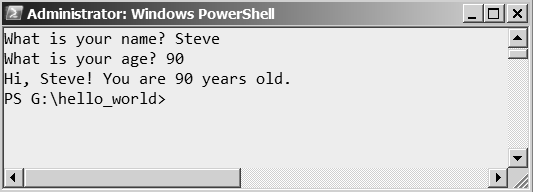
\includegraphics[width=.90\textwidth]{/Chapter3/Figure_16}
\end{figure}

\section{Comparison operators}

Python recognizes a number of comparison operators that we can use to evaluate expressions:

\begin{figure}[h]
	\caption{Python comparison operators}
	\centering
\begin{center}
	\begin{tabular}{|c | c|}
		\hline Operator & Description \\ [0.5ex]
		\hline
		\textless & Less than \\
		\hline
		\textgreater & Greater than \\
		\hline
		\textless = & Less than or equal to \\
		\hline
		\textgreater = & Greater than or equal to \\
		\hline
		== & Equal to \\
		\hline
		!= & Not equal to \\ [1ex]
		\hline
	\end{tabular}
\end{center}
\end{figure}

Comparisons constructed using these operators will return a boolean value of either \texttt{true} or \texttt{false}. See the example in Figure 3.21.

\begin{figure}[h]
	\caption{Using logical and comparison operators}
	\begin{lstlisting}
	print(5>6)	# prints false
	print(6<5)	# prints true
	print(6==5)	# prints false
	print(6!=5)	# prints true
	print("foo"="foo")	# prints true
	print("foo"!="bar")	# prints true
	\end{lstlisting}
\end{figure}

\section{Conditional statements}

So far the programs that we have written have been pretty simple in that every line of code has been executed in a sequential order. However, we can also write programs with have branching paths that only execute based upon the result of an internal test. For example, perhaps we are writing a program that will ask the user a different set of questions dependent on whether they identify as a man or a woman. We can write such a program by using conditional statements. The simplest form is an \texttt{if} statement which evaluates a boolean expression and executes one or more commands if the evaluation returns true. This is usually paired with an \texttt{else} statement that executes if the evaluation returns false. See the example in Figure 3.22.

\begin{figure}[h]
	\caption{Using the \texttt{if} statement}
\begin{lstlisting}
age = input("What is your age? ")
if(age >= 18):
	print("Congratulations!")
	print("You are old enough to vote in the United States!")
else:
	print("Sorry!")
	print("You are not old enough to vote in the United States!)
\end{lstlisting}
\end{figure}

This simple program accepts numeric input from the user and stores the response in a variable called \texttt{age}. It then prints a different response depending on whether the numeric value is greater than or equal to 18. 

It is important to note that including a colon (:) after the \texttt{if} and \texttt{else} statements is required. In addition, all lines after the colon that are indented the same amount will be executed if the \texttt{if} or \texttt{else} statement is triggered.

Sometimes a program may need to consider more than two possibilities. In this case we can use the conditional statements \texttt{elif} which stands for ``else if". An example of how to use \texttt{elif} is presented in Figure 3.23.

\begin{figure}[h]
	\caption{Using the \texttt{elif} statement}
	\begin{lstlisting}
	favNumber = input("Can you guess my favorite number?")
	if (favNumber==5):
		print("Correct! 5 is my favorite number!")
	elif (favNumber==4):
		print("No! 4 is my least favorite number!)
	else:
		print("Wrong!")
	\end{lstlisting}
\end{figure}

This program contains three branches. One is executed if the user inputs the number 5, another if the user inputs the number 4, and the third if the user inputs any other number.

\section{Logical operators}

Conditional statements can be paired with logical operators to create more complex comparisons. The three logical operators that Python supports are \texttt{and}, \texttt{or}, and \texttt{not}. See Figure 3.24 for an example of how these operators can be used with a conditional statement:

\begin{figure}[h]
	\caption{Logical operators}
\begin{lstlisting}
	age = input("What is your age? ")
	if(age >= 21):
		print("You are old enough to vote and drink alcohol.")
	elif(age >=18) and (age < 21):
		print("You are old enough to vote but not to drink alcohol.")
	else:
		print("You are not old enough to vote or drink alcohol.")
\end{lstlisting}
\end{figure}

\section{Iteration}
While we have learned how to write programs that contain branching paths, our programs so far have been limiting to executing each instruction a single time. However, we will likely want to develop programs that have the capability to use the same code some specified number of times. In order to do this we need to learn about iteration, which is an incredibly important computer programming concept to understand.

The basic idea is straightforward. We start with a test that returns a boolean result of either \texttt{true} or \texttt{false}. If the result is \texttt{true}, our program executes a block of code. Afterwards, the program evaluates the original test again. If the result is still \texttt{true}, the code block executes again. The program continues to loop through the code until the test returns a value of \texttt{false}.

The simplest type of iterative loop is called the \texttt{while} loop. An example program that uses this \texttt{while} as well as sample output are presented in Figures 3.25 and 3.26.

\begin{figure}[h]
\caption{An example using the \texttt{while} loop.}
\begin{lstlisting}
keepRunning = "yes"
while (keepRunning == "yes"):
	keepRunning = keepRunning("Should the program keep running? ")
print("Ok, I'll stop the program. Bye!")
\end{lstlisting}
\end{figure}

\begin{figure}[h]
	\caption{Output for an example using the while loop}
	\centering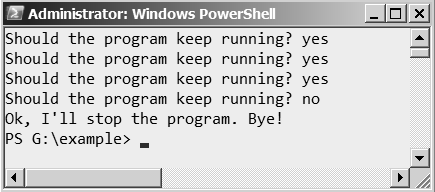
\includegraphics[width=.90\textwidth]{/Chapter3/Figure_26}
\end{figure}

Let's work our way through this example. The program first declares a variable \texttt{keepRunning} which holds the string \texttt{yes}.\footnote{In this book we'll be using the Lower CamelCase convention for naming our variables and functions. This means that when several words are joined together, the first letter of the first word is lowercase but the first letters for subsequent words are uppercase. Naming conventions in programming are primarily an aesthetic choice; however they do sometimes generate heated debate.} It then evaluates the expression to the right of the \texttt{while} command which tests whether the value of \texttt{keepRunning} is \texttt{yes}. This expression initially evaluates as \texttt{true} so the program enters the loop. Within the loop, the program prompts the user to answer the question \texttt{"Should the program keep running"?}. Note that the value of \texttt{keepRunning} is then overwritten with the input the user provides. Since there are no more lines of code within the block, the program re-evaluates the expression to the right of the \texttt{while} command. If the expression still evaluates as \texttt{true} (i.e., \texttt{keepRunning} still holds the string \texttt{yes}) then the program enters the loop as well and the process repeates. If the expression evaluates as \texttt{false}, the program skips over the loop and prints \texttt{"Ok, I'll stop the program. Bye!"}. Note that, in this example, the code within the loop could theoretically execute an infinite number of times so long as the user keep entering in the string \texttt{yes} when prompted.

There also may be times where we want a program to execute over a loop some predetermined number of times. In this case, we would want to use a different type of iterative loop called a \texttt{for} loop. An example of a program using this type of loop (as well as the respective output) is provided in Figures 3.27 and 3.28.

\begin{figure}[h]
	\caption{An example using the \texttt{for} loop.}
	\begin{lstlisting}
	for i in range(0,3):
		print("We've run through the loop " + str(i++) + " time(s).")
	print("Bye!")
	\end{lstlisting}
\end{figure}

\begin{figure}[h]
	\caption{Output for an example using the for loop}
	\centering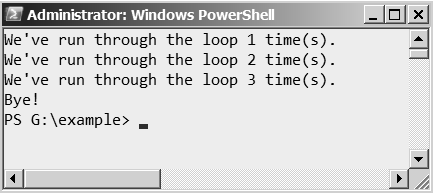
\includegraphics[width=.90\textwidth]{/Chapter3/Figure_28}
\end{figure}

The first line of code declares a new variable, \texttt{i}. The command \texttt{in range(0,3)} then tells Python to iterate over a sequence that contains 3 items beginning with 0 (i.e., the sequence 0, 1, 2). To begin, \texttt{i} is initially assigned the value of the first item in the sequence (\texttt{0}). The program then enters the loop. Within the loop, the message \texttt{We've run through the loop X time(s)!} is displayed, with X representing the value of \texttt{i+1}. Note that if we instructed Python to simply display the value \texttt{i} instead of \texttt{i+1}, the user would see the sequence 0, 1, 2 instead of 1, 2, 3. As discussed earlier in the chapter, we also need to tell Python to convert \texttt{i} to a string using \texttt{str()}. The loop then executes again, this time with \texttt{i} taking the value of the next item in the sequence (1). When finished, the program then iterates through the sequence one final time (i = 2) before breaking out of the loop and displaying the \texttt{Bye!} message.

\section{Searching for help}
As a novice programmer, you will frequently encounter situations where you need a bit of help. Your first stop for help should usually be the latest version of the Python documentation which can be found at \texttt{https://docs.python.org/3}. As the ``authoritative guidance" prepared by the Python Foundation, you can be assured that this documentation is up-to-date and accurate.

Search engines such as Google\texttrademark , can also be helpful tools for finding answers to your programming problems. However, you should be aware that many online programming websites have weak or non-existent methods for quality control. Thus, you should attempt to verify that any source code you plan to adopt into your own programs comes from a reputable source.\footnote{Certain websites, such as Stack Overflow\texttrademark , have adopted a community rating feature which allegedly prioritizes high quality responses to user questions.}
\section{Summary}
This chapter began by presenting a brief background of the Python programming language and then discussed how to set up a simple development environment. Common data types were presented as well as functions for displaying output and accepting user input. Constructing conditional statements using comparison and logical operators was also introduced. The chapter concluded with a discussion of iteration using both \texttt{for} and \texttt{while} loops.

\section{Exercises}
\begin{enumerate}
		\item Indicate the data type for each of the following expressions (your choices are bool, int, str, or float):
	\begin{enumerate}
		\item 3
		\item 3.0
		\item s
		\item -3
		\item True
		\item bar
	\end{enumerate}
	\item Indicate the output that would be returned from each of the following expressions:
	\begin{enumerate}
		\item "pythonrocks"[1]
		\item "pythonrocks"[2]
		\item "pythonrocks"[:2]
		\item "pythonrocks"[2:]
	\end{enumerate}
	\item Indicate the output that would be returned from each of the following expressions:
	\begin{enumerate}
		\item 6 \textgreater = 4
		\item 3 != 3
		\item 2 \textgreater 1
	\end{enumerate}
	\item Indicate whether each of the following expressions would evaluate as \texttt{true} or \texttt{false} assuming the variable \texttt{foo} is previously declared as \texttt{foo = 12}:
	\begin{enumerate}
		\item if (foo == 13) or (foo == 12)
		\item if (foo == ``12")
		\item if (foo not 12)
		\item if (foo == 12) and (foo == 13)
		\item if (foo not 13)
	\end{enumerate}
	\item How would you write the following code more efficiently using a \texttt{for} loop?
	\begin{lstlisting}
	print(2)
	print(4)
	print(6)
	print(8)
	print("Bye!")
	\end{lstlisting}
	
	\item Write a program that takes the age of the user and converts it to dog years (you can assume that one dog year is equivalent to one human year). For example, if you are 98 years old in human years that means you are 14 years old in dog years.
	\item Write a program that takes a user's weight (in kilograms) and height (in centimeters) and calculates their Body Mass Index (BMI). Based upon their BMI, the program should then indicate whether the user is considered underweight (BMI of 18 or less), normal weight (BMI of greater than 18 but less than 26) or overweight (BMI of 26 or greater). Note that the formula for calculating BMI is weight/height\textsuperscript{2}.
	
	As a check, the BMI for a user with a height of 180cm and 70kg would be 21.6.
	\item Write a program that takes the users name and displays it back in reverse order. For example, if the user indicates that her name is \texttt{Sarah}, the program should print the name \texttt{haraS}.
	\item Modify the program in Figure 3.27 so it prints the messsage \texttt{"We've run through..."} a specific number of times requested by the user. Note that the \texttt{input()} function you have learned about assigns using the string data type and that strings can be converted to integers using the function \texttt{int()}.
	\item Write a program that takes a user's name and iterates over each letter in the name using a \texttt{for} loop. For each round of iteration, your program should print the message \texttt{Letter X of your name is "A"}, where X represents the position of the letter and A represents the letter itself.
	
	For example, if the user entered the name \texttt{Tom}, the program would output:
	
	\texttt{Letter 1 of your name is T\\Letter 2 of your name is o\\Letter 3 of your name is m}
	\item Write a program that translates the user's name into Pig Latin. English words are translated into pig latin by taking the first letter of the word, moving it to the end of the word, and adding "ay". For example, the name "Steve" in Pig Latin would become "Tevesay."
	\item \textbf{Portfolio project:} The \textit{Fibonacci sequence} is an integer sequence identified by 13th century mathematician Leonardo of Pisa that is characterized by the fact that every number after the first two is the sum of the two proceeding ones. The first ten items in the sequence are: \texttt{1, 1, 2, 3, 5, 8, 13, 21, 34, 55}.
	
	Write a Python program that displays the first 25 numbers in the \textit{Fibonacci sequence}. Each line of output should display both the number itself and its position in the sequence. For example:\\ \\
	\texttt{1:	1} \\ \texttt{2:  1} \\ \texttt{3:  2} \\ \texttt{4:  3...}
	\\ \\ As a check, the 15th number in the Fibonacci sequence is 610 and the 25th number is 75,025.
	\item \textbf{Portfolio project:} Write a program that guesses a secret number. The program should contain the following features:
	\begin{itemize}
		\item It should ask the user to think of a number between 0 and 100.
		\item It should guess what the number is and prompt the user to indicate whether the guess was too high, too low, or correct.
		\item It should repeat the preceding step until the user indicates that the number is correct.
		\item It should display an error message if the user enters a command that the program does not recognize.
	\end{itemize}
	As an example, your program's output might look something like:
	\begin{figure}[h]
		\centering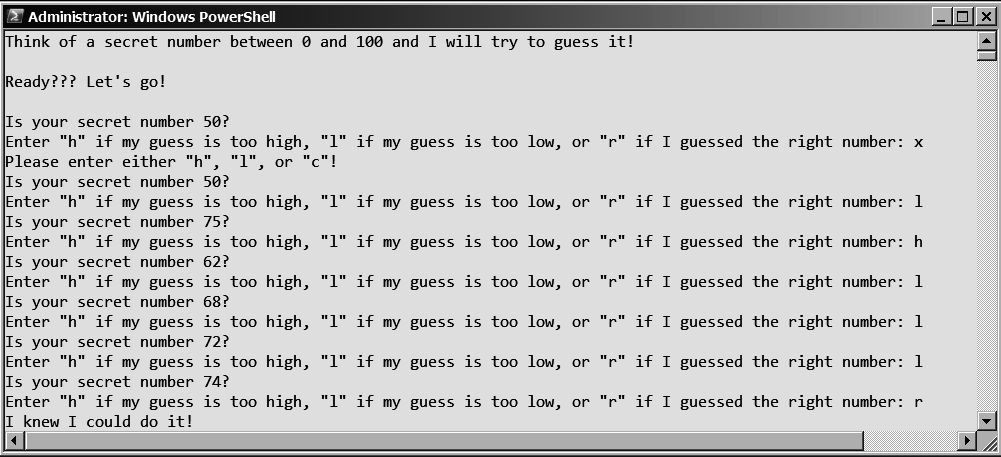
\includegraphics[width=.90\textwidth]{/Chapter3/Exercise}
	\end{figure}

	Hint: Remember that you can round floats to the nearest integer by using the function \texttt{int()}.	
\end{enumerate}

\chapter{Intermediate Python concepts}
\section{Introducing functions}
When writing Python programs, we will often to write code that can be reused in a variety of different circumstances within the program. We can do so by defining functions. An example of a Python function and the related program output is provided in Figures 4.1 and 4.2.
\begin{figure}[h]
\caption{A function example}
\begin{lstlisting}
	def PrintInitials(firstName, lastName):
		print(firstName[0] + "." + lastName[0])
	
	firstName = input("What is your first name? ")
	lastName = input("What is your last name? ")
	print("Your initals:", end=" "), PrintInitials(firstName, lastName)
	print("Tom Smith's initials:", end=" "), PrintInitials("Tom", "Smith")
\end{lstlisting}
\end{figure}

Let's break down the syntax for this function.

\begin{itemize}
	\item First, we tell Python to define a new function called \texttt{PrintInitials} using the command \texttt{def}.
	\item We thenn tell the function to expect two arguments each time it is called, \texttt{firstName} and \texttt{lastName}. 
	\item We end the function definition with a colon \texttt{I}. 
	\item We write the specific code that the function should execute (each line of code must be indented to be attached to the function).
\end{itemize}

\begin{figure}[h]
	\caption{Output for a function example}
	\centering\includegraphics[width=.90\textwidth]{/Chapter4/Figure_1}
\end{figure}

Now whenever we want to call this specific function, we simply call it by name and encapsulate the specific argument values we want to pass in parentheses separated by a comma. The program presented in Figure 4.1 provides an example of passing variable as arguments, \texttt{PrintInitials(firstName, lastName)}, as well as specific strings, \texttt{PrintInitials("Tom","Smith)}.\footnote{This program also contains a simple "hack" to make sure that the initials are printed on the same line as the preceding text. While the \texttt{print("")} function normally appends a newline character at the end of its output, the keyword argument \texttt{end = " "} tells the function to append a space instead.} Be aware that all arguments in Python are passed by reference. This means that if you change the value of a variable passed as an argument within a function, the value also changes for any other part of your program that has access to that variable.

When writing functions, we can also use the \texttt{return} expression to pass an argument back when the function exits. For example, the function presented in Figure 4.3 calculates the user's initials in a new variable called \texttt{initials} which is returned to the calling function \texttt{print()}.

\begin{figure}[h]
	\caption{A example using \texttt{return}}
	\begin{lstlisting}
	def ReturnInitials(firstName, lastName):
		initials = firstName[0] + "." + lastName[0] + "."
		return initials

	firstName = input("What is your first name? ")
	lastName = input("What is your last name? ")
	print("Your initals are", end=" ")
	print(ReturnInitials(firstName, lastName))

	\end{lstlisting}
\end{figure}

\section{Global versus local variables}
It is important to understand that variables which are defined inside a function body have what is called \textit{local scope}. This means that these variables can only be accessed by code contained within the function itself. Conversely, variables which have \textit{global scope} can be accessed by the entirety of the program. Figure 4.4 provides an example of declaring variables with local versus global scope.

\begin{figure}[h]
	\caption{Global versus local scope}
	\begin{lstlisting}
	myGlobalVar = "Hello!" # a global variable
	def myFunction():
		myLocalVar = "Hello!" # a local variable
		return myVar
	
	print myGlobalVar # prints "Hello!" 
	print myLocalVar # exception - variable is out of scope
	
	\end{lstlisting}
\end{figure}

\section{Lists}
All of the programming examples we have reviewed so far have involved simple types of data (primarily numbers and strings). However, we will often encounter programming problems where we need to structure different types of data together in complex ways using compound data types. The first compound data type we will review is called the \texttt{list}. Lists are simply containers of data elements that are organized from first to last. We can declare lists using the following syntax:

\texttt{numbers = [1, 2, 3, 4, 5]} \\
\texttt{animals = ["cow", "mouse", "horse", "pig"]} \\
\texttt{prices = [1.99, 2.99, 3.00, "free", 9.99]}

As you can see, the contents of lists are placed within brackets and separated by commas. Lists can store any of the types of data that we have learned about so far (such as \texttt{string}, \texttt{int}, and \texttt{float}) and can even store combinations of different data types. 
We can then access individual elements with a list by referring to the specific index we want to access, similar to the string indexing method we learned about in Chapter 2.

\texttt{numbers[0]} returns the integer \texttt{1}\\
\texttt{animals[1]} returns the string \texttt{mouse}\\
\texttt{prices[2:4]} returns a list containing the float \texttt{2.99} and the string \texttt{free}.

We can also use the \texttt{for loops} that we learned about in Chapter 2 to iterate over the elements in a list. For example, the code presented in Figure 4.5 prints the elements of two lists using iteration. 

\begin{figure}[h]
	\caption{Lists and iteration}
	\begin{lstlisting}
	animals = ["cow", "mouse", "horse", "pig"]
	numbers = [1, 2, 3, 4, 5]

	for i in animals:
		print(i);

	for i in numbers:
		print(str(i))
	\end{lstlisting}
\end{figure}

We can also create lists that have more than one dimension. For example, let's say we wanted to create a list of X and Y coordinates. We could initialize such a list as follows:

\texttt{coords = [[1, 2], [1, 7], [2, 3]]}
	
If we then wanted to access the first set of coordinates (1, 2) we could type:

\texttt{coords[0]}

By nesting our bracketed terms, we can access specific elements within a multidimensional list. For example, if we wanted to access a specific coordinate within a set (for example, the Y coordinate 7 from the second set of coordinates) we could type:

\texttt{coords[1][1]}

It's also important to understand that lists are mutable. This means that we can assign a new value to a list after it has been created. For example, if we wanted to change the value of the first element in a list, we could do so using the assignment operator as follows:

\texttt{myList[0] = "foo"}

Python also supports a large number of manipulation methods for lists that are worth reviewing. A brief description of some of these methods is provided below.

\begin{itemize}
	\item len(): Returns the number of elements in a list.
	\\ \texttt{len(myList)}
	\item append(): Adds a new element after the last element in a list.
	\\ \texttt{myList.append("qux")}
	\item pop(): Removes the last element from a list. If an index is provided within parentheses, this method will remove that specific element from a list.
	\\ \texttt{myList.pop() \\ myList.pop(1)}
	\item insert(): Inserts a new element into a list at the index provided 
	\\ \texttt{myList.insert(1, "foo")}
	\item remove(): Removes the first element in the list which contains the value specified 
	\\ \texttt{myList.remove("foo")})
	\item index(): Find the index for the first occurance of an element in a list.
	\\ \texttt{myList.index("foo")}
	\item sort(): Sort in ascending numeric or alphabetical order (list elements must be either entirely numeric or entirely string).
	\\ \texttt{myList.sort()}
\end{itemize}

\section{Dictionaries}
Dictionaries are similar to lists in that they can contain elements of various data types. However, while the indices of lists are required to be integers (e.g., 1, 2, 3), dictionaries can have indices (specifically referred to as "keys") of any type. A dictionary is really just a data structure that contains a collection of these key-value pairs. 

Dictionaries are initialized using curly braces, values are preceded by colons, and key-value pairs are separated by commas. After initialization, specific values in the dictionary can be referenced by using their respective key. The code example and output provided below demonstrate the concept (see Figures 4.5 and 4.6)

\begin{figure}[h]
	\caption{A simple dictionary}
	\begin{lstlisting}
	gradePoints = {"A": 4.0, "B": 3.0, "C": 2.0, "D": 1.0, "F": 0.0}
	print(gradePoints["A"])
	print(gradePoints["B"])
	print(gradePoints["C"])
	print(gradePoints["D"])
	print(gradePoints["F"])
	\end{lstlisting}
\end{figure}

\begin{figure}[h]
	\caption{Output for the simple dictionary example}
	\centering\includegraphics[width=.90\textwidth]{/Chapter4/Figure_6}
\end{figure}

This program creates a dictionary which assigns grade point values to keys representing university letter grades. Each grade point value is then accessed by reference to its respective letter. 

It is important to note that we should never try to access a key that doesn't exist,  For example, if we modified the code above to include the line \texttt{print(gradePoints["E"])}, Python would generate an error and halt the program. This can be prevented by using a conditional expression to confirm that a key exists prior to attempting to access its value:

\texttt{if "E" in gradePoints: print (gradePoints["E"])}\\
\texttt{else: print ("Grade not found.")}

We can loop through dictionaries to obtain keys and corresponding values by using the \texttt{items.()} method. Figure 4.8 demonstrates this concept. 

\begin{figure}[h]
\caption{Iterating over a dictionary}
\begin{lstlisting}
	employees = {"Name": "Steve", "Job": "Accounting professor", "Age": 90}
	
	for k, v in employees.items():
	print (k + ": " + str(v))
\end{lstlisting}
\end{figure}

This program prints of the key-value pairs in the \texttt{employees} dictionary. During iteration, the name each key is stored in the variable \texttt{k} while the related value is stored in the variable \texttt{v}. Note also that, since \texttt{v} contains integer values in this example, it needs to be passed as a string using \texttt{str()} to the \texttt{print()} function.

Dictionary values can also be easily changed by referencing their related key: \\ \texttt{employees["Name"] = "Bob"}

New key-value pairs can by using the assignment operator: \\ \texttt{employees["Weight"] = 150}

Finally, key-value pairs can be deleted from a dictionary by using the \texttt{del} statement:

\texttt{del employees["Age"]}

Be warned that it can be dangerous to make significant changes to dictionaries since the content will change for other functions that reference the same dictionary. Before modifying a dictionary's contents, consider whether it would be more useful to create a modified copy of the dictionary. The \texttt{copy()} method can be used to create a dictionary copy as follows:

\texttt{employees2 = employees.copy()}
\section{File input and output}
While we have already learned how to create programs which can collect data input from a user, the programs we will write to handle accounting data will often need to be able to read/write data from/to a file. Python 3+ incorporates a number of handy i/o functions and methods that can make working reading and writing files fairly simple.

To begin, let's create a new file:

\texttt{myFile = open("myFile.txt", "w", newline="")}

This function creates a new file object called \texttt{myFile} which points to the path of the file to be opened (\textbackslash myFile.txt). The second paramater (\texttt{"w"}) tells Python to open the file for writing. If we omit the second parameter, Python assumes that are simply opening an existing file for reading only. In this case, if the file does not exist, Python will generate an error. The final parameter \texttt{newline=""} is required for properly formatting a CSV file on Windows-based systems.

Once we have created a new file object, we can modify the file by using the \texttt{write()} method as follows:

\texttt{myFile.write("Mary had a little lamb")}

This line of code will append the string \texttt{Mary had a little lamb} to the file referenced by the myFile object. This method will also return the number of characters contained in the string (including spaces) which can be useful when checking for errors. 

Python contains many methods that can be used to read data from a file. We can read the entire contents from a file using the \texttt{read()} method as follows:

\texttt{newFile.read()}

Or we can read a single line from a file using \texttt{readline()}:

\texttt{newFile.readline()}

We can also read lines from a file one at a time by iterating over the file object as follows:

\texttt{for line in newFile:   print(line, end="")}

However, reading entire lines of data is often not terribly useful. You may normally find yourself wanting to read individuals data elements which are separated by some specific delimiting character, such as a space or a comma. For example, let's assume that we want to write a program that reads a file \texttt{names.txt} which contains the following data:

\texttt{sam bob julie steve rachel}

We want our program to read each of the names in the file individually and store them in a list called \texttt{nameList}. The code snippet presented in Figure 4.9 demonstrates how this program might be written.

\begin{figure}[h]
\caption{Reading a space delimited file}
\begin{lstlisting}
	file = open("names.txt")
	names = []

	for line in file:
		for word in line.split(" "):
			names.append(word)

	print("The contents of the names list are:")
	print(names)
	file.close()
	\end{lstlisting}
\end{figure}

This program begins by opening the \texttt{names.txt} file. Note that we have omitted the second parameter from the \texttt{open()} function because we want Python to open the file for reading only. Next, we create an empty list \texttt{names} which will store the data elements that we read from the \texttt{names.txt} file.

We then use a pair of nested \texttt{for} loops to read each name individually. The first loop simply iterates over each line in the file. However, the second loop iterates over each \textit{word} in the line by splitting the line into individual segments delimited by the space character (" "). Each word read is then added to the list using the \texttt{append()} method that we discussed earlier. Finally, the program print the new contents of the \texttt{names} list data structure. If we wanted, we could then access individual items of the list by referencing its specific index (e.g., \texttt{print(names[0])}.

When we are done writing to the file, we need to call \texttt{.close()} to close the file and free up the system resources taken up by the file object. Note that any references your program makes to a file object after it has been closed will fail. 

\section{Reading and writing data using JSON}

While the methods that we have learned about so far are useful for reading and writing simple data, they have some drawbacks. First, the \texttt{read()} and \texttt{write()} methods only work with string data types. Therefore, numeric values would need to be converted to a different data type, using a function like \texttt{int()}, if they need to be manipulated. In addition, these simple methods are really not very convenient when trying to read/write more complex data structures like lists or dictionaries. 

Thankfully, Python supports the ability to save more complicated data types using the JSON (Javascript Object Notation) data interchange format. JSON is commonly used by many different types of applications so adding support for it into your programs can be quite useful (you can read more about the JSON format at \texttt{https://wwww.json.org}).

To encode an object using JSON, we pass the data to be encoded as well as an open file object to the \texttt{dumps()} function. Data encoded in the JSON format can be decoded by using the \texttt{load()} function. An example of a simple program which demonstrates the use of these functions is presented in Figure 4.10.

\begin{figure}[h]
	\caption{Reading and writing using JSON}
	\begin{lstlisting}
	import json
	
	names = ["sam", "bob", "julie", "steve", "rachel"]
	newNames = []
	
	file = open("names.json", "a")
	
	json.dump(names, file)
	file.close()
	
	file = open("names.json")
	newNames = json.load(file)
	print("The contents of newNames is:")
	print(newNames)
	file.close()
	\end{lstlisting}
\end{figure}

A brief review of this code is in order. The first line of the program imports the \texttt{json} module which allows us to use Python's JSON-specific encoding/decoding functionality.\footnote{You can think of Python modules as simply collections of source code which can provide access to additional Python functionality. We'll be using many different Python modules as we advance through this text}. The program then creates a list called \texttt{names} which contains five elements. It also initializes an empty list called \texttt{newnames}. A new file object (called \texttt{file}) is then initialized and mapped to the path \texttt{\textbackslash names.json} (the .json file extension is typically used to denote JSON-encoded data files). Note that the program passes the \texttt{"a"} parameter since \texttt{names.json} is a new file that will be written to.

The program then calls the \texttt{dump} function which is part of the \texttt{json} module, as discussed earlier. The first argument passed to the function is the name of the list we wish to write, while the second argument represents the name of the file object to be written to. On line 9, the program closes the \texttt{file} object and removes it from memory. At this point, if we viewed the working directory of our program, we would see that, in addition to our Python script, it now contains a file called \texttt{names.json}.

The program then creates a brand new file object and associates it with the \texttt{\textbackslash names.json} file path. Note that the \texttt{"a"} argument has been omitted from the call to the open function because we want Python to open an existing file for reading only (this is the default function call). The program then uses the \texttt{load} function from the \texttt{json} module to load the contents of the \texttt{names.json} file to the empty \texttt{newNames} list. The program then prints the contents of \texttt{newNames} to ensure that the JSON data was successfully decoded. Finally, the program closes the file object and removes it from memory.

\section{Advanced: Classes}

So far we have learned about various types of data as well as how to create various functions to manipulate that date. You can perhaps imagine that it might be helpful if there were a way to somehow bundle together certain types of data, as well as their related functions into a single unitary package. 

Python is an example of what is called an \textit{object oriented programming language}. As such, Python allows us to create unique data structures (called classes) which contain both data and specific functions that interact with that data (called interfaces). These classes are essentially blueprints for creating specific data types (called objects) that contain the data types and functions specified in the classes. This probably all sounds very confusing but I promise that it will become more clear as we talk through the following example.

Imagine we have been hired to develop a simple program for tracking a client's accounts receivable. The specifications that the client has for this program are relatively simple:

\begin{itemize}
	\item Each invoice added to the program should be assigned a unique invoice number
	\item For each invoice, the program should keep track of the customer name, the amount due, and whether the invoice has been paid
	\item The program must provide the ability for users to modify the amount due on the invoice
	\item The program must provide the ability for users to display the customer name, amount due, and payment status on demand
\end{itemize}

As we begin, we need to think carefully about how this program is going to store the invoice data that it is responsible for keeping track of. For example, we could store the invoice number as an integer varaiable called \texttt{invoiceNo}, the customer's name in a string called \texttt{customer}, the amount owed in a float called \texttt{amount}, and the payment status (paid or upaid) in a boolean variable called \texttt{paid}. We would then also need to think about creating functions that would allow the user to modify the amount due, set the payment status, and to display the attributes of each invoice. Perhaps we could call these functions \texttt{modifyAmount()}, \texttt{setPaid()}, and \texttt{display()}, respectively.

Obviously, each invoice will need its own set of variables and functions. So how might we keep track of which variables and functions are assigned to each invoice? Well, we could adopt a naming convention which would allow the specific invoice to be inferred from a variable/function name (e.g., \texttt{inv1\_customer}. \texttt{inv2\_customer}, \texttt{inv3\_setPaid()}, etc.) This makes conceptual sense but keeping track of all of these variables and functions would become unmanageable as the number of invoices grows in size. In addition, this approach would generate an enormous amount of repetitive code.

Since all invoices have essentially the same set of attributes, it would be much easier to instead develop a blueprint (called a ``class'') which describes the specific variables and functions that are needed by each invoice. Then every time a new invoice needs to be created, we can use this blueprint to create an instance of the class (called an ``object'') which represents the specific invoice. Let's review Figure 4.11 for an example of how this might work.

\begin{figure}[h]
	\caption{A simple program for tracking accounts receivable}
	\begin{lstlisting}
	class Invoice:
		"Common base class for invoices"
		invoiceNoCounter = 0
	
		def __init__(self, customer, amount):
			self.customer = customer
			self.amount = amount
			Invoice.invoiceNoCounter += 1
			self.invoiceNo = Invoice.invoiceNoCounter
			self.paid = False
	
		def changeAmount(self, amount):
			self.amount = amount
	
		def setPaid(self):
			self.paid = not self.paid
	
		def display(self):
			print("Customer: " + self.customer, end =", ") 
			print("Invoice #: " + str(self.invoiceNo), end = ", ")
			print("Amount: " + str(self.amount), end = ", ")
			print("Paid: " + str(self.paid))
	
	invoice1 = Invoice("Acme Company", 1541.99)
	invoice2 = Invoice("XYZ Inc.", 4750.15)
	invoice1.display()
	invoice2.display()
	invoice1.setPaid()
	invoice2.changeAmount(4500.99)
	invoice1.display()
	invoice2.display()
	\end{lstlisting}
	
\end{figure}

To create a class, we use the \texttt{class} statement followed immediately by the name of the class that we wish to create (in this case, we are creating a new class called \texttt{Invoice}. All of the code associated with the class definition is then indented after this initial statement.

The first line of the class definition (line 2 in Figure 4.11) is reserved for the class's ``documentation string.'' This is simply a variable with a string type that typically contains a brief description of the class. The exact contents of the documentation string are entirely up to you.\footnote{The document string is stored in the class variable \texttt{\_\_.doc\_\_}}

Line 3 of the program initializes a new variable \texttt{invoiceNoCounter}. This variable is referred to as a ``class variable" because it will be shared by all instances of the class. The purpose of this variable is track the number of invoices that have been recorded in the system for purposes of assigning each invoice a unique invoice number. This variable is initially assigned a value of 0.

On line 5 we define a class function called \texttt{\_\_init\_\_}. Functions that are defined within class definitions are referred to as ``methods" and we will be using this terminology from this point forward. The double underscores before and after the method name indicates that this is a special name reserved by the Python interpreter. The \texttt{\_\_init\_\_} method contains code that will be executed each time time a new instance of a class is created. Every class definition you create should contain a \texttt{\_\_init\_\_} method. 

Note that the \texttt{\_\_init\_\_} method within our Invoice class has three arguments. The first argument, \texttt{self}, is always included as the first argument for any class method that you create. \texttt{self} is simply an identifier used to refer to a specific instance of a class. Be advised that you do not have to specifically pass the self argument when calling a function, Python will implicitly pass it for you. The second paramter, \texttt{customer}, will take the name of the customer associated with a specific invoice being created. The final parameter, \texttt{amount}, will take the dollar amount of the invoice being created. The body of the \texttt{\_\_init\_\_} method takes the later 2 parameter values and assigns them to two new instance variables called \texttt{customer} and \texttt{amount}, respectively (variables defined within a class that are shared with class instances are refereed to as ``members.") The prefex \texttt{self} indicates that the new members should be initialized uniquely for each specific instance of the class. This ensures that each class instance will have its own unique \texttt{customer} and {amount} members.

The third line of the \texttt{\_\_init\_\_} method (Line 8) increments the \texttt{invoiceNoCounter} class variable which we declared earlier by 1. Recall that class variables are shared by all instances of the class, which we reference this variable using the class name \texttt{Invoice}. The fourth line of the method assigns this value to a new member \texttt{invoiceNo}. The \texttt{self} prefix indicates that this variable will be created uniquely for each instance of the class. The final line of the method creates a new instance member called \texttt{paid} which will indicate whether the invoice has been paid. This member is assigned an initial value of \texttt{False}.

Line 12 defines a new class method \texttt{changeAmount} which is used to change the value of an invoice object. The method takes the value passed as \texttt{amount} and assigns it to a new instance member of the same name. 

Line 15 defines a new class method \texttt{setPaid} which toggles the value of the \texttt{self.paid} data member. Note that the expression \texttt{not self.paid} returns the inverse of the current value of \texttt{self.paid} (i.e., if the current value of \texttt{self.paid} is \texttt{true}, the expression returns \texttt{false}.) Finally, the class method \texttt{display} defined on line 18 prints the value of the instance's members.

With the class definition complete, we can new create individual instances of the class. Let's review the expression included in line 24 of the program and repeated below:

\texttt{invoice1 = Invoice("Acme Company", 1541.99)}

This statement object called \texttt{invoice1} which has a class type of \texttt{Invoice}. Remember that the  \texttt{\_\_init\_\_} method is called when an instance of a class is created, that this method takes three arguments, and that Python automatically passes the first argument \texttt{self} for us. This means that Python expects us to pass a value for the remaining \texttt{customer} and \texttt{amount} arguments when initializing the object. In the code above, the string \texttt{Acme Company} is passed as the \texttt{company} argument and \texttt{1541.99} is passed as the \texttt{amount} argument. ]

The remaining lines of the program call various other object methods. For example, the call to \texttt{invoice1.setPaid()} on Line 28 toggles the \texttt{paid} data member within the \texttt{invoice1} object. The call to \texttt{invoice2.setamount} on Line 29 passes the value \texttt{4500.99} as the argument \texttt{amount} which is used to update the value of the \texttt{invoice2.amount} data member. Finally, the calls to the \texttt{display} method display the value of the data members for each object. The output that would be displayed upon running the full program is presented in Figure 4.12.

\begin{figure}[h]
	\caption{Output for the AR tracking program}
	\centering\includegraphics[width=.90\textwidth]{/Chapter4/Figure_12}
\end{figure}

\section{Advanced: Inheritance}

In the previous section, we created a simple Python class definition for creating invoice objects. This class contained data members for an object's invoice number, customer name, amount, and payment status as well as specific methods for accessing and manipulating those members. 

Suppose that our client is happy with our work so far and has now asked us to modify our Python program to also track accounts \textit{payable} invoices. Our revised program should share many of the features of our previous program to track accounts receivable invoices: it should store the payables invoice number, whether it has been paid, and should provide the ability to modify payable amounts, update the paid status, and display the invoice attributes. 

\begin{figure}[h]
	\caption{The parent invoice class}
	\begin{lstlisting}
	class Invoice:
		"Common base class for invoices"
		invoiceNoCounter = 0
	
		def changeAmount(self, amount):
			self.amount = amount
	
		def setPaid(self):
			self.paid = not self.paid
	
		def display(self):
			print("Customer/Vendor: " + self.company, end =", ") 
			print("Invoice #: " + str(self.invoiceNo), end = ", ")
			print("Amount: " + str(self.amount), end = ", ")
			print("Paid: " + str(self.paid))
	\end{lstlisting}
\end{figure}

We could start from scratch and create a new class definition for accounts payable invoices. However, we could instead modify our original invoice class to contain only data members and methods that are common across all invoice objects. We could then create two derived classes from this parent invoice class that relate to accounts payable and accounts receivable invoices specifically. These derived classes would inherent the common attributes from the parent class. The example in Figure 4.13 demonstrates how the parent class could be defined, while the derived classes are presented in Figure 4.14.

Note that the parent \texttt{Invoice} class is very similar to the version of the class presented earlier. It still contains a class variable for ensuring that accounts receivable invoices contain a unique ID number. It also has methods to change the amount of the invoice, set the payment status, and display the invoice attributes.  Note that we modified the \texttt{display} method slightly due to the fact that the company listed on a receivables invoice would be referred to as the ``customer,'' while the company listed on a payables invoice would be referred to as the ``vendor.''

\begin{figure}[h]
	\caption{The derived classes}
	\begin{lstlisting}
	class AccountsReceivable(Invoice):
		"Derived class for accounts receivable invoices"
		def __init__(self, customer, amount):
			self.company = customer
			self.amount = amount
			Invoice.invoiceNoCounter += 1
			self.invoiceNo = Invoice.invoiceNoCounter
			self.paid = False
	
	class AccountsPayable(Invoice):
		"Derived class for accounts payable invoices"
		def __init__(self, vendor, amount, invoiceNo):
			self.company = vendor
			self.amount = amount
			self.invoiceNo = invoiceNo
			self.paid = False
	\end{lstlisting}
\end{figure}

Derived classes are declared similarly to their parent class; however the parent class to be inherited from is identified in parentheses after the class name. Both derived classes will share all of the same methods as the \texttt{Invoice} parent class, with the exception of the \texttt{\_\_init\_\_} which has been overriden in each of the derived class definitions. This is due to the fact that we want our accounts payable and accounts receivable objects to be initialized with different arguments. For example, note that initializing an \texttt{AccountsPayable} object requires the passing of an \texttt{invoiceNo} argument which is assigned to \texttt{self.invoiceNo}, while initializing the \texttt{AccountsReceivable} object assigns a \texttt{self.invoiceNo} value generated from the parent class \texttt{Invoice.invoiceNoCounter}. This is due to the fact that invoice numbers for the AR invoices should be generated internally, while the invoice numbers for the AP invoices need to be supplied by the vendors.

For an example of how these derived classes could be instantiated and how to call their methods, carefully review the following code excerpt and the related output presented in Figure 4.15. 

\texttt{invoice1 = AccountsReceivable("Acme Company", 1541.99) \\
invoice2 = AccountsPayable("XYZ Inc.", 4750.15, 2833303) \\
invoice1.display() \\
invoice2.changeAmount(4500.99) \\
invoice2.display()} 

\begin{figure}[h]
	\caption{Output for the modified invoice tracking program}
	\centering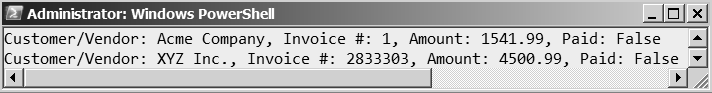
\includegraphics[width=.90\textwidth]{/Chapter4/Figure_15}
\end{figure}

\section{Summary}

We began this chapter by introducing functions, which are useful programming tools for writing reusable code. We then discussed lists and dictionaries, which are commonly used data structures for handling more complex data. We learned the basic steps involved in saving to and reading from files, including encoding/decoding using the JSON format. The chapter concluded with an introductory discussion of object oriented programming concepts including classes and inheritance.

\section{Exercises}
\begin{enumerate}
		\item What is the difference between local versus global scoping of variables? Why do you think programmers generally prefer to avoid using variables with global scope?
	\item Assume that we've created a list with the following assignment: \\ \texttt{var myList = [1, 4, ["foo", 3, "bar"], "baz"]}
	\\Specify the output that would be returned by each of the following expressions:
	\begin{enumerate}
		\item \texttt{myList[0]}
		\item \texttt{myList[2]}
		\item \texttt{myList[:3]}
		\item \texttt{myList]-2]}
		\item \texttt{myList[2][2]}
		\item \texttt{myList[::]}
		\item \texttt{4 in x}	
		\item \texttt{myList.len()}
		\item \texttt{myList.index(4)}
	\end{enumerate}
	\item Assume that we've created a list with the following assignment: \\ \texttt{var myList = [1, 4, ["foo", 3, "bar"], "baz"]}
	\\Indicate how \texttt{myList} would look after calling each of the following methods (assume the methods are called sequentially).
	\begin{enumerate}
		\item \texttt{myList.pop()}
		\item \texttt{myList.index(1, "bar")}
		\item \texttt{myList.append("qux")}
		\item \texttt{myList.remove(1)}
		\item \texttt{myList.sort()}
	\end{enumerate}
	\item The following code stub starts the definition of a class called \texttt{JournalEntry}. Objects instantiated using this definition should have the members \\ \texttt{accountName} and \texttt{amount}. Complete the code stub by replacing the commented code \texttt{\#Line 1} and \texttt{\#Line 2}.
	
	\texttt{class JournalEntry: \\ \mbox{~~~~}def \_\_init\_\_(self, accountName, amount): \\ \mbox{~~~~~~~~}\#Line 1: Create a member for the account name \\ \mbox{~~~~~~~~}\#Line 2: Create a member for the journal entry amount}
	\item In Exercise 3.6 you were asked to write a program which displays the first 25 numbers in the \textit{Fibonacci sequence}. Modify this program so that this calculation and related printout is encapsulated in a function. The function should take a single parameter, \texttt{num}, which is specified by the user and indicates the number of elements in the sequence to print. 
	
	\item Write a program that will ask the user to enter a temperature in Fahrenheit and prints the temperature in Celsius. The program should contain a function which takes a single argument, \texttt{farTemp}, and returns the converted temperature. Note that the conversion formula is \textit{C = (F - 32) * (5/9)}. As a check, 76 degrees Farenheit is equivalent to approximately 24 degrees Celsius.
	
	\item Write a function that combines two lists of identical length by alternating each element and returns the combined list. For example, if the first list is \texttt{["foo", "bar", "baz", "qux"]} and the second list is \texttt{[1, 2, 3, 4]}, the function would return \texttt{["foo", 1, "bar", 2, "baz", 3, "qux", 4]}.
	
	\item Write a function that takes two lists and return a new list that contains only the unique values from both lists. For example, if the first list is \texttt{[1, 2, 3, 4]} and the second list is \texttt{[6, 5, 4, 3]}, the function would return \texttt{[3, 4]}.
	
	\item Create dictionary that contains a series of keys representing abbreviations of five US states (e.g., NY, MA, CA) whose related valuates are the city capitals of each state (e.g., New York City, Boston, Sacramento). Write a program that will prompt the user to enter the abbreviation of a US state. If the user enters the abbreviation of a state included in the dictionary, the program should print that state's capital. If the state is not included in the dictionary, the program should return a message indicating that fact.
	
	\item \textbf{Portfolio project:} Write a simple program that creates a database of your friends' birthdays. The program should give the user the options to 1) add a new friend and birthday to the database, 2) remove a friend and birthday from the database, 3) change the birthday for a friend already included in the database, 4) print the current friends and birthdays stored in the database, and 5) export the contents of the database to a JSON file. You should use conditional statements to manage user input. You may want to consider using a dictionary as the organizational structure supporting your database.
	
	\item \textbf{Portfolio project:} The file \texttt{wordlist.txt} posted on the textbook website contains a list of 69,903 English words. Using this word list, create a game of Hangman using Python. The program should read the word list file and randomly choose a single word from the list. It should then provide the user with a limited number of chances to guess individual letters that make up the word. An example of what such a program might look like is presented in Figure 4.16.
	
	\begin{figure}[h]
		\caption{Sample program output for exercise 7}
		\centering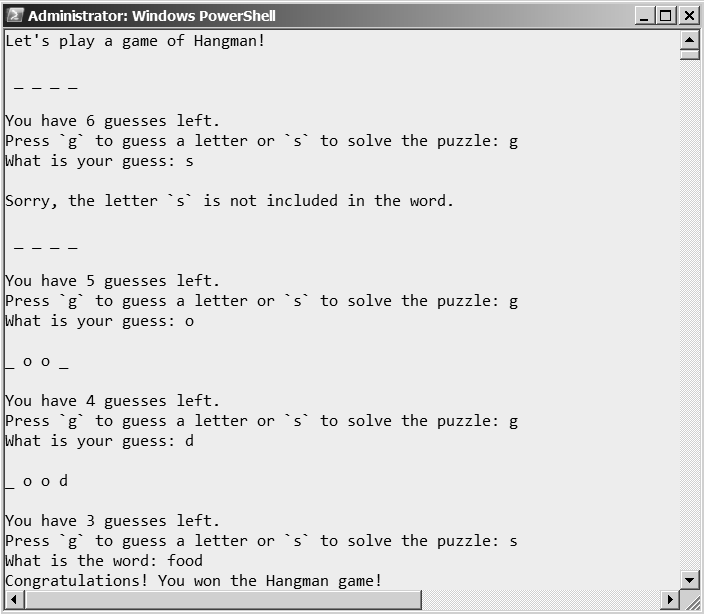
\includegraphics[width=.80\textwidth]{/Chapter4/Exercise_7}
	\end{figure}

	Hint: To help choose a random word from the list provided, consider using the \texttt{randint()} function which is provided as part of Python's \texttt{random} module. For example, \texttt{"number = random.randint(1,10)} will assign a random number between 1 and 0 to the variable \texttt{number}.
	
	\item \textbf{Portfolio project:} Modify the example in Figure 4.11 so that it is interactive and also keeps track of a new invoice attribute - the payment due date. The user should have the ability to manually add new invoices and display the attributes of invoices that have already been entered. Hint: You will likely want to use a list data structure to store the invoice objects your program generates. For a further challenge, add the ability to delete specific invoices (it may be helpful to review some of the standard Python list methods that were discussed earlier in the chapter).
\end{enumerate}

\chapter{Collecting data from the web}
	Websites often contain useful data for performing accounting analytic tasks. For example, a client may post certain relevant accounting data on an internal corporate website, or an auditor may want to gather pricing data from the external website of a vendor for purposes of performing valuation test work. Thankfully, it is relatively easy to write Python programs that can gather data from the web.
	
\section{A brief overview of HTML}
	
	HTML is an acronym that stands for HyperText Markup Language. You can think of HTML as essentially a programming language for displaying information in a web browser. It is comprised of a collection of short statements (referred to as ``tags'') which tell the browser how website content should be presented to the viewer. At their most basic level, tags can apply simple formatting to website text. For example, the tag \texttt{<b>} can be used to make text appear bolded. Within a webpage's HTML document, this tag could be used as follows:
	
	\texttt{Hello! <b> This text is bolded </b> but this text is not.}
	
	If a web browser were to then read this line of HTML code, it would display the following:
	
	Hello! \textbf{This text is bolded} but this text is not.
	
	Note that HTML tags are always encapsulated in angle brackets and the closing tag is always prefaced with a forward slash (/). HTML contains a wide variety of tags that can be used to display information in a myriad of different ways, such as including information in tables, or in graphics and videos. A brief list of some common HTML tags is presented in Figure 5.1. For our purposes, learning about HTML in great depth is beyond the scope of this book\footnote{That being said, understanding HTML can be an invaluable skill for a budding data scientist. For beginners, I recommend Jon Duckett's book \textit{HTML and CSS: Design and Build Websites} which is published by John Wiley \& Sons.} That being said, once we understand how information used in a particular website is tagged, we can use that knowledge to gather data that is of interest to our analyses. For example, if we were interested in obtaining all of the information that is displayed on a website in \textbf{bolded} text, we could write a Python program that reads the website's HTML code and saves any data encapsulated in \texttt{<b>} tags. This is commonly referred to as ``web scraping''.

\begin{figure}[h]
	\caption{Common HTML tags}
	\centering
	\begin{center}
		\begin{tabular}{|c | c|}
			\hline Tag & Description \\ [0.5ex]
			\hline
			\texttt{<HTML>} & The entire HTML document \\
			\hline
			\texttt{<HEAD>} & The header of the document \\
			\hline
			\texttt{<TITLE>} & The title of the document \\
			\hline
			\texttt{<BODY>} & The body part of the document \\
			\hline
			\texttt{<P>} & A paragraph \\
			\hline
			\texttt{<DIV>} & A custom container unit \\
			\hline
			\texttt{<H1>} & A section heading (subheadings are \texttt{<H2>} through \texttt{<H6>}) \\
			\hline
			\texttt{<IMG>} & An image \\
			\hline
			\texttt{<LI>} & A list item \\
			\hline
			\texttt{<TABLE>} & A table \\
			\hline
			\texttt{<TR>} & A table row \\
			\hline
			\texttt{<TD>} & A data cell for a table \\
			\hline
			\texttt{<THEAD>} & The header for a table \\
			\hline
			\texttt{<TH>} & A header cell for at table \\
			\hline
			\texttt{<A>} & A hyperlink \\
			\hline
		\end{tabular}
	\end{center}
\end{figure}

\section{Necessary libraries}
	
	We will be writing our web scraper using the free Python library \textit{Beautiful Soup} written by Leonard Richardson. The project's website, which includes the latest release and documentation, is located at:
	
	\texttt{https://www.crummy.com/software/BeautifulSoup/}
	
	To give Python the ability to access the web and pass HTML data to \textit{Beautiful Soup}, we'll be using the free Python library \textit{Requests}. The website for the library, which also includes the latest release and documentation, is located at:
	
	\texttt{http://docs.python-requests.org/en/latest}
	
	We'll be using the Python package management system, \textit{Pip} to install both libraries. \footnote{If you're using Python version 3.4 or later, \textit{Pip} should already be installed on your machine. You can verify this by by typing \texttt{pip} from your terminal console. If for some reason \textit{Pip} is not installed on your system, you can follow the installation instructions available at \texttt{https://docs.python.org/3/installing/}} \textit{Pip} allows Python packages to be installed using the command:
	
	\texttt{pip install package-hame}
	
	In our case, we'll be running the following two commands within PowerShell to install \textit{Beautiful Soup} and \textit{Requests}:
	
	\texttt{pip install beautifulsoup4} \\
	\texttt{pip install Requests}
	
	If the packages have installed correctly, \textit{Pip} should display output similar to Figures 5.2 and 5.3.
	
\begin{figure}[h]
	\caption{Successful installation output for \textit{Beautiful Soup}}
	\centering\includegraphics[width=.80\textwidth]{/Chapter5/Figure_1}
\end{figure}

\begin{figure}[h]
	\caption{Successful installation output for \textit{Requests}}
	\centering\includegraphics[width=.80\textwidth]{/Chapter5/Figure_2}
\end{figure}

\section{Viewing a webpage's HTML code}
	Prior to scraping the data from a web page, we need to understand how the data on that particular page is being tagged. We can do that by viewing the page's HTML source code within a web browser. In this example, we'll be scraping a website that contains a fictional company's ending inventory information. You'll note that this website lists inventory data across a series of three individual webpages which can be navigated using hyperlinks in the lower-left corner of the page. This website can be found at:
	
	\texttt{http://www.steveperreault.com/textbook.inventory1.html}
	
	Once you've navigated to the site, right click anywhere in the browser frame and open the \textit{Inspector} pane, as demonstrated in Figure 5.4. The inspector tool allows us to see the underlying HTML code for any portion of a webpage that we click on. \footnote{The option to select this tool may look slightly different if you are using another browser; in this case we are using Google Chrome.\texttrademark}
	
	\begin{figure}[h]
		\caption{The \textit{Inspector} menu option}
		\centering\includegraphics[width=.80\textwidth]{/Chapter5/Figure_3}
	\end{figure}

	Activate the selection tool from within the \textit{Inspector} pane (see Figure 5.5) and then click on any of the tabular inventory data contained in the browser pane. The \texttt{Inspector} page will change to display the HTML code associated with the inventory data (see Figure 5.6).
	
\begin{figure}[h]
	\caption{The \textit{Inspector} selection tool}
	\centering\includegraphics[width=.95\textwidth]{/Chapter5/Figure_4}
\end{figure}

\begin{figure}[h]
	\caption{The HTML source for the inventory data table}
	\centering\includegraphics[width=.95\textwidth]{/Chapter5/Figure_5}
\end{figure}

	You will notice that the inventory table as a whole is encapsulated within \texttt{<table>} tags. Individual rows of a table are contained within \texttt{<tr>} tags. The first row of the table represents the header and is enclosed within \texttt{<thead>} tags and contains five cells for the table headings, each enclosed within \texttt{<th>} tags. The body of the table is encapsulated within \texttt{<tbody>} tags. Finally, cells containing standard data are enclosed within \texttt{<td>} tags. This is the standard scheme for tagging tabular data in an HTML document. 

\section{Building a basic webscraper using Python}

	Now that we understand how the data we are interested in has been tagged, we can write a Python program to collect that data using \textit{Beautiful Soup} and \textit{Requests}. To keep things understandable, we'll develop the application slowly in individual pieces. 
	
	First, we need to tell Python to import the \textit{Requests} module so we have access to the tools we need to access the web. 
	
	\texttt{import requests}
	
	Now, let's create a new variable, called \texttt{url} which will store the address of the webpage we want to scrape (represented as a string).
	
	\texttt{url = "http://www.steveperreault.com/textbook/inventory1.html"}
	
	Next, we will call the \textit{Requests} method \texttt{get} which will return webpage data from the address we provide. We'll pass the \texttt{url} variable we just created to this method and store the returned data into a new object called \texttt{response}.
	
	\texttt{response = requests.get(url)}
	
	The HTML content of the webpage is stored in a method called \texttt{content}. We can verify that the object was created correctly by printing the contents of that method as follows.
	
	\texttt{print (response.content)}
	
	If we've done everything correctly, running this program should display the raw HTML from the webpage we are attempting to scrape, similar to that shown in Figure 5.7. While this is a good first step, we now need to modify the program to strip out the extraneous information, including the HTML tags, and display only the data we are interested in. \textit{Beautiful Soup} has several helpful methods that will aid us in this effort. 
	
\begin{figure}[h]
	\caption{Raw HTML data}
	\centering\includegraphics[width=.95\textwidth]{/Chapter5/Figure_8}
\end{figure}	
	
	First, let's modify our program to also import the \textit{Beautiful Soup} methods we need. Note that the \texttt{from} prefix ensures that we are importing from the \texttt{bs4} module which is compatible with Python version 3+.
	
	\texttt{from bs4 import BeautifulSoup}
	
	We'll then create a new \textit{Beautiful Soup} object from the \texttt{requests} object that was created earlier.
	
	\texttt{soup = BeautifulSoup(response.content)}
	
	This new \texttt{soup} object contains all of the HTML presented in the original document (you can \texttt{print()} its contents to verify this). We're only interested in capturing the data contained within the table and, as we learned earlier, that data is encapsulated within \texttt{<tbody>} tags. We can use the \texttt{find()} method to identify only data contained with the \texttt{tbody} tag and save that into a new object called \texttt{table}.
	
	\texttt{table = soup.find("tbody")}
	
	We will then call the object's \texttt{prettify()} method which formats the content by placing each HTML tag on its own line. Then we'll print out the contents of the \texttt{table} object so we can see what we've collected so far.
	
	\texttt{table.prettify()} \\
	\texttt{print(table)}
	
	Again, if we've done everything correctly, the output of our program should look similar to that presented in Figure 5.8. Note that the program has only captured the data contained within the \texttt{tbody} tags -- all of the other HTML code has been removed from the object.
		
\begin{figure}[h]
	\caption{"Prettified" table data}
	\centering\includegraphics[width=.95\textwidth]{/Chapter5/Figure_9}
\end{figure}

	Remember that within our table body, rows are identified by the \texttt{<tr>} tag, while individual data cells are identified by the \texttt{<td>} tag. We want to take the data within each of these cells and store it in a data structure that can then be accessed and manipulated by Python. Thankfully, the list data structure that we learned about in Chapter 4 is perfect for storing tabular data. Let's go ahead and create a new list called \texttt{inventory} now.
	
	\texttt{inventory = []}
	
	We now need to tell our Python program to grab the data that is contained in the \texttt{table} object and place it into our new \texttt{inventory} list structure. Specifically, the program should read through the \texttt{table} object and, every time it encounters the \texttt{<tr>} tag, it should make a new row in the \texttt{inventory} list. Then, when it encounters data encapsulated within \texttt{<td>} tags, we want it to copy that data as a new element into the \texttt{inventory} list. This process should proceed until Python has processed the entire \texttt{table} object.
	
	This sounds just like an iterative process which means we'll be able to apply the iteration concepts from Chapter 3. The specific loop we'll want to include in our program is presented in Figure 5.8.

\begin{figure}[h]
\caption{Copying data to a list}
\begin{lstlisting}
for row in table.findAll("tr"):
	rowContents = []
	for cell in row.findAll("td"):
		rowContents.append(cell.string)
	inventory.append(rowContents)
\end{lstlisting}
\end{figure}	

Note the first expression uses \textit{Beautiful Soup's} \texttt{findAll} method to tell Python to iterate over all of the rows in the table which are identified by the \texttt{<tr>} tag. When a new row is found, the program then initializes a new list called \texttt{rowContents} which will be used to store the data elements in that row. On line 3, a second \texttt{for} loop is used to iterate over all of the cells in the row chich are identified by the \texttt{<td>} tag. Every time a new cell is encountered, its content (contained within the \texttt{string} member) is appended to the end of the \texttt{rowContents} list. Finally, when all the cells in a row have been processed, \texttt{rowContents} is appended to the \texttt{inventory} list. The process then starts again for the next row in the table. 

After the completion of this process, the \texttt{inventory} list data structure should contain the inventory data that were are interested in. If we were to display its contents, the output would look similar to that presented in Figure 5.10.

\begin{figure}[h]
	\caption{Contents of \texttt{inventory} list data structure}
	\centering\includegraphics[width=.95\textwidth]{/Chapter5/Figure_10}
\end{figure}

It is likely the case that we will want to save the contents of our list to a file so they can be used in other programs. We could write the code to do this ourself, iterating over the elements in the list and saving each to a text file (we learned how to do this in Chapter 4) However, Python contains a handy built-in module called \texttt{csv} which can more easily output the contents of our \texttt{inventory} data structure into a comma-delimited format. We're going to use this module now to save us some code.

First, we'll import the module, create a new file object called \texttt{output} and associate the file object with the file \texttt{inventory.csv}\footnote{\texttt{.CSV} is the common file extension for comma-delimited files.} Recall that the \texttt{a} parameter ensures that a new \texttt{inventory.csv} will be created if one does not exist already. This was covered earlier in Chapter 4.

\texttt{import csv} \\
\texttt{output = open("inventory.csv", "w", newline="")}

We then call the \texttt{writer} method which will create a new object {writerObj} that will be used to write data to the file object we just created.

\texttt{writerObj = csv.writer(output)}

Finally, the method \texttt{writerows} is used to write all the rows in the \texttt{inventory} list to the CSV file we specified.

\texttt{writerObj.writerows(inventory)}

Executing this program will create a new file in our working directory \texttt{inventory.csv} which contains a comma delimited list of all of the inventory data from the website. We can open the file in a spreadsheet program such as Microsoft Excel\texttrademark to verify that its contents.

There is still one last thing that we're missing - the table headers. Recall that we only told \textit{Beautiful Soup} to parse data within \texttt{<tbody>} tags; however, the table's column headers are contained within \texttt{<thead>} tags. We could write some additional code to tell \texttt{Beautiful Soup} to gather that data for us and then add it to the \texttt{inventory.csv} file following the steps we just reviewed. However, unless you are working with a table that has a very large number of columns, it is often easier to simply insert the table headers into the CSV file manually. We can do this using the \texttt{writerow} method which will write a single row of data to the \texttt{inventory.csv} file. Be sure to make this call prior to writing the rest of the tabular data to the file.

\texttt{writerObj.writerow(["Warehouse", "SKU", "Desc", "onHand", "Price"])}

The full source code for the program so far and the related CSV file (as viewed in Microsoft Excel) are presented in Figures 5.11 and 5.12, respectively.

\begin{figure}[h]
\caption{A basic web scraper}
\begin{lstlisting}
	import requests
	from bs4 import BeautifulSoup
	import csv

	url = "http://www.steveperreault.com/textbook/inventory1.html"

	response = requests.get(url)

	soup = BeautifulSoup(response.content)

	table = soup.find("tbody")

	inventory = []

	for row in table.findAll("tr"):
		rowContents = []
		for cell in row.findAll("td"):
			rowContents.append(cell.string)
		inventory.append(rowContents)

	output = open("inventory.csv", "w", newline="")
	writerObj = csv.writer(output)
	writerObj.writerow(["Warehouse", "SKU", "Desc", "onHand", "Price"])
	writerObj.writerows(inventory)
\end{lstlisting}

\end{figure}

\begin{figure}[h]
	\caption{The contents of \texttt{inventory.csv}}
	\centering\includegraphics[width=.95\textwidth]{/Chapter5/Figure_12}
\end{figure}

\section{Scraping multi-page websites}

While the program we have written does an excellent job scraping a single webpage, our inventory list is not yet complete. Recall that the complete inventory list is spread across a series of three sequentially numbered webpages(\texttt{inventory1.html, inventory 2.html,} and \texttt{inventory3.html}) and that the scraper we have written only collects the data included on the first page.\footnote{It is often the case that, when webpages contain data which spans across multiple pages, the webpage names will be numbered sequentially}.

We could address this issue creating three separate programs that each contain modified versions of the \texttt{url} string which point to the three webpages we want to gather data from. However, there is a more elegant solution to this problem which uses iteration to grab the data that we need. 

Let's first modify the string \texttt{url} as follows:

\texttt{url = "http://www.steveperreault.com/textbook/inventoryX.html"}

We'll then encapsulate the code which gather ands writes the data to the \texttt{inventory} list within a \texttt{for} loop which we will set to run a series of three times (once for each webpage we want to gather data from): 

\texttt{for i in range(1,4):}

Each time the loop executes, we will use string indexing to create a new url string (\texttt{newUrl}) which replaces the \texttt{X} character with the iteration count as follows:

\texttt{newUrl = url[0:-6] + str(i) + url [-5:]}

Note that this expression is slicing the \texttt{url} string six spaces before the end (i.e., removing \texttt{.html} portion), inserting the iteration count which is held in the integer \texttt{i}, and then appending the last five characters of \texttt{url} (\texttt{.html}) to the end of the new string. 

There's a couple of additional changes we need to make. First we need to move the list constructor \texttt{inventory = []} outside of the loop because we don't want it to be overwritten each time the loop iterates. In addition, we need to make sure that the creation of the \texttt{writerObj} object and calls to its methods occur after the loop has finished executing. This is because we only want to write the \texttt{inventory} list structure to the \texttt{CSV} file after the data has been fully collected. 

The complete and final source code for our basic webscraper is presented in Figure 5.13.

\begin{figure}[h]
	\caption{A basic web scraper with support for loading multiple webpages}
	\begin{lstlisting}
	import requests
	from bs4 import BeautifulSoup
	import csv
	
	url = "http://www.steveperreault.com/textbook/inventoryX.html"
	
	inventory = []
	
	for i in range(1,4):
		newUrl = url[0:-6] + str(i) + url[-5:]
		print("Gathering data from " + newUrl)
		response = requests.get(newUrl)
		soup = BeautifulSoup(response.content)
	
		table = soup.find("tbody")
	
		for row in table.findAll("tr"):
			rowContents = []
			for cell in row.findAll("td"):
				rowContents.append(cell.string)
				inventory.append(rowContents)
	
	output = open("inventory.csv", "w", newline="")
	writerObj = csv.writer(output)
	
	writerObj.writerow(["Warehouse", "SKU", "Desc", "onHand", "Price"])
	writerObj.writerows(inventory)
	\end{lstlisting}
	
\end{figure}

\section{Summary}
The chapter begin with a discussion of common HTML tags and reviewed how the HTML code of a webpage can be viewed. It then discussed how to use the \textit{Beautiful Soup} and \textit{Requests} libraries to build a simple Python program to scrape tabular data from single-page websites. Use of iteration to scrape from multi-page websites was also discussed.

\section{Discussion Questions}
\begin{enumerate}
	\item What does HTML stand for? What do the terms that make up this acronym refer to?
	\item Imagine you are developing a web scraper and want to all of the image data contained within a webpage. How would you modify the code presented in Figure 5.13 to gather such data?
\end{enumerate}
\section{Exercises}
\begin{enumerate}
	\item \textbf{Portfolio Project}: Develop your own interactive web scraper. The program should prompt the user to type a URL address and then generate a CSV file which contains all tabular data contained within the page. Test that your program works by finding a webpage that contains data in tabular form and providing it to the program you have written. 
	
	Wikipedia, in particular, is a rich source of tabular HTML data. A few examples of Wikipedia pages containing such data are:
	
	\begin{itemize}
		\item List of cities by population \\ https://en.wikipedia.org/wiki/List\_of\_cities\_proper\_by\_population
		
		\item List of countries by median age\\
		https://en.wikipedia.org/wiki/List\_of\_countries\_by\_median\_age
		
		\item List of countries by labor force size \\
		https://en.wikipedia.org/wiki/List\_of\_countries\_by\_labour\_force
		
	\end{itemize}
	
	 
\end{enumerate}

\chapter{Working with tabular data}

\section{Installing Pandas}
We'll be using the \textit{Python Data Analysis Library} (Pandas) module to help us analyze tabular data. Pandas adds data frame functionality to Python, similar to what is included in languages such as R. Data frames are similar to the traditional spreadsheets that you are familiar with, in that they allow for mixed data types to be presented within labeled rows and columns. Pandas also contains a wide variety of analysis tools that are useful in accounting analytics contexts. The project's website, which includes the latest release and documentation, is located at:

\texttt{https://pandas.pydata.org}

Similar to how we have previously installed other Python modules, we'll be installing Pandas from with Powershell using the command:

\texttt{pip install pandas}

In addition to Pandas, the installer should also install the numpy module, upon which Pandas is based. When writing code that will use Pandas functionality, we will always need to import both modules as follows:

\texttt{import pandas as pd \\ import numpy as np}

\section{Constructing data frames manually}
A data frame is simply a table with labeled rows and columns. Let's imagine that we want to create a data frame using the inventory data that we collected in the previous chapter. We would begin by first creating a dictionary where each column in our table is included as a key along with a corresponding list of values (refer back to Chapter 4 for a discussion of dictionaries). For example:

\texttt{data = \{"sku": ["EN876923", "EN687311"], "qty": [106, 49]\}}

We can then create the data frame by calling the \texttt{DataFrame} function and passing the dictionary as well as a list representing the headers for each row:\footnote{The \texttt{pd} prefix to the \texttt{DataFrame} function indicates that we are calling the function contained within the Pandas namespace. This prefix should always be used before calling a Pandas function.}

\texttt{inventory = pd.DataFrame(data, index=["Warehouse A", "Warehouse B"])}

If we then print out the \texttt{table} data frame, we would see the following:

\begin{figure}[h]
	\caption{Creating a data frame manually}
	\centering\includegraphics[width=.90\textwidth]{/Chapter6/Figure_1}
\end{figure}

\section{Constructing data frames from .CSV}
Of course, you will rarely want to create a data frame manually. Rather, you will typically populate your data frames using an external source, such as a CSV file. Let's create a new data frame from the \texttt{inventory.csv} data file we prepared in the previous chapter. To do so, we would call Pandas' \texttt{read\_csv} function as follows:

\texttt{inventory = pd.read\_csv("inventory.csv")}

Note that, by default, Pandas will assign sequential numeric row headers, similar to a typically spreadsheet. These header values are referred to as the data frame's "index."

\section{Printing data frames}
Like other data types, Pandas data frames can be printed to the screen by passing them to the \texttt{print()} function. We may occasionally want to print a portion of a frame to screen to ensure that it has been set up properly. To avoid printing the entire contents of the data frame, we can call the \texttt{head()} which, by default, returns the first five rows of data. \texttt this method can also take the parameter \texttt{n=X}, where X represents a custom number of rows to be printed.

\section{Changing frame indices}

Any column within a data frame can become the frame's index by using the \texttt{reset\_index()} and \texttt{set\_index()} functions. By passing the \texttt{drop=True} parameter to \texttt{reset\_index} we remove the existing sequential numeric index from the data frame. We then call \texttt{set\_index} with the name of the column header representing the new index as the sole parameter. 

For example, let's say we want to index our \texttt{inventory} data frame by the name of the warehouse the inventory is located in. This could be done with the following expression:

\texttt{newInventory = inventory.reset\_index(drop=True).set\_index("Warehouse")}

To verify that our re-indexing worked as intended, we could print the first five rows of the new data frame as follows:

\texttt{print(new.Table.head())}

The respective output is presented in Figure 6.2.

That being said, modifying a data frame's index can present some problems if we try to transform our data frames in the future. As a result, we'll stick with the original sequential numeric index for the examples presented in this chapter.

\begin{figure}[h]
	\caption{Re-indexing a data frame}
	\centering\includegraphics[width=.90\textwidth]{/Chapter6/Figure_2}
\end{figure}

\section{Sorting data}

Data frames can be sorted by index using \texttt{sort\_index()}. This method will sort in ascending order; however a frame can be sorted in descending order by passing the \texttt{ascending = False} parameter. By default, the method returns a new data frame, however you can tell Pandas to sort and overwrite the existing data frame by passing \texttt{inplace = True}. For example:

\texttt{inventory.sort\_index(inplace=True, ascending=False)}

Pandas can sort data frames by data value using the \texttt{sort\_values()} method and passing the header of the column to sort by. For example, if we wanted to sort the \texttt{inventory} data frame by price, we could use the following expression:

\texttt{inventory.sort\_values("Price", inplace=True, ascending=False)}

\section{Arithmetic operations}

Pandas also provides support for the four basic arithmetic operations (addition, subtraction, multiplication, and division). Let's say that we want to take the \texttt{onHand} and \texttt{Price} columns from the \texttt{inventory} data frame, multiply the two, and create a new column that represents the extended price. 

\texttt{inventory["Ext"] = inventory.Price * inventory.onHand}

Note that the term in brackets represents the header for the new column and the and the calculation is performed using the standard Python multiplication operator. Other arithmetic operations can be performed using the various other operators. The output for this example if provided in Figure 6.3.

\begin{figure}[h]
	\caption{Arithmetic operations}
	\centering\includegraphics[width=.90\textwidth]{/Chapter6/Figure_3}
\end{figure}

\section{Aggregating data}
When working with accounting information, we will often find the need to summarize or aggregate data. For example, perhaps we want to group sales of individual products by category or summarize the value of journal entries affecting a particular account. Pandas contains a function called \texttt{groupby()} which allows us to perform this task easily. We just need to pass the the column to aggregate by as well as an aggregation function which can be selected from the options presented in Figure 6.4.

\begin{figure}[h]
	\caption{A sample of common \texttt{groupby()} aggregation functions}
	\centering
	\begin{center}
		\begin{tabular}{|c | c|}
			\hline Function name & Description  \\ [0.5ex]
			\hline
			\texttt{sum()} & Sum the numerical rows in the group \\
			\hline
			\texttt{prod()} & Multiply the numerical rows in the group \\
			\hline
			\texttt{mean()} & The average of the numerical rows in the group \\
			\hline
			\texttt{count()} & The number of rows in the group \\
			\hline
		\end{tabular}
	\end{center}
\end{figure}

For example, let's say we want to identify the total quantity of inventory items contained in the \texttt{newInventory} data frame across all warehouses. Since each item has a unique SKU number, we could use \texttt{groupby()} to aggregate inventory by this identifier and aggregate the sum of the grouped items to a new dataframe. We would use the following expression:

\texttt{sumInventory = inventory.groupby("SKU").sum().reset\_index()}

Note that this requires us to also reset the numeric sequential index to fit the new data frame using \texttt{reset\_index}. Omitting this call will default to using the first column of data as the index, which could present problems with transforming the frame going forward.

Printing the \texttt{sumInventory} data frame would yield the output presented in Figure 6.4.

\begin{figure}[h]
	\caption{Aggregation output}
	\centering\includegraphics[width=.90\textwidth]{/Chapter6/Figure_4}
\end{figure}

\section{Merging data frames}
Note that the contents of the \texttt{sumInventory} data frame omit the project description and warehouse name. This is because both values are non-numeric and, thus, cannot be aggregated using the \texttt{sum()} aggregation function. Fear not - we insert the description of each SKU back into \texttt{sumInventory} by merging it with the \texttt{newInventory} data frame.

The \texttt{merge()} method can easily be used to combine rows that share a common index. As parameters, it takes the two frames to be merged, and the name of the column to be used to perform the match. If the column index has the same name within both names, you can simply pass that name, as follows:

\texttt{table = pd.merge(frame1, frame2, on="index")}

If the column index has a different name, you can specify the name of the index to be used as follows:

\texttt{table = pd.merge(frame1, frame2, left\_on="index1", right\_on="index2")}

Note that, within this expression, the left and right keys refer to the first and second parameters passed to the method, respectively.

With this knowledge, we can now merge the contents of the \texttt{sumInventory} and \texttt{inventory} frames into a new data frame as follows:

\texttt{sumInventoryExt = pd.merge(inventory, sumInventory, on="SKU")}

Printing the output of sumInventoryExt will return the following:

\begin{figure}[h]
	\caption{Merge output with duplicates}
	\centering\includegraphics[width=.90\textwidth]{/Chapter6/Figure_5}
\end{figure}

A review of this output indicates that this is not quite what we want. It seems like each row of \texttt{sumInventoryExt} contains multiple columns for the \texttt{onHand}, \texttt{Price}, and {Ext} variables and that Pandas has attached either a \texttt{\_x} or \texttt{\_y} suffix to these columns. This is because the \texttt{sumInventory} data frame contains the inventory listing at the summarized level, while \texttt{inventory} does not. As a result, Pandas cannot find key matches within these three columns across the data frame and so it includes data from both frames when creating \texttt{sumInventoryExt}. This is not helpful to us, so let's do something about it.

\section{Deleting data and removing duplicates}

Let's create a new data frame called \texttt{skuList} which contains only a listing of individual SKU numbers and their respective conditions. We'll build this new frame from the \texttt{inventory} frame, eliminating the data that we don't need using the following commands:

\texttt{skuList = inventory.drop("Warehouse", 1)\\
skuList.drop("Price", 1, inplace = True)\\
skuList.drop("onHand", 1, inplace = True)\\
skuList.drop("Ext", 1, inplace = True)\\}

The first expression creates a new data frame which is set to the same value of the \texttt{inventory} frame with the \texttt{Warehousn} column removed. The parameter \\texttt{1} which is passed to the \texttt{drop} method tells Pandas that \texttt{Warehouse} is a column label (passing a value of 0 would denote a row label). The next three lines of code remove the remaining unneeded columns from the \texttt{skuList} frame. Recall that the parameter \texttt{inplace = True} tells Pandas that the existing \texttt{skuList} frame should be modified.

Alternatively, we could construct the new frame \texttt{skuList} and simply include only the \texttt{SKU} and \texttt{Desc} columns from the \texttt{inventory} frame as follows:

\texttt{skuList = inventory[["SKU","Desc"]]}

Either way, the end result is a new data frame called \texttt{skuList} which includes only two columns labeled \texttt{SKU} and \texttt{Descr}. However, this new frame still contains a large number of duplicate rows which we should remove using the \texttt{drop\_duplicates()} method.

\texttt{skuList = skuList.drop\_duplicates().reset\_index(drop=True)}

Note that we also use the \texttt{reset\_index()} method to drop the old index and build a new one based upon the new number of rows in the data frame.

Printing out this new table should result in output similar to Figure 6.7, which represents a list of unique inventory SKUs and their related descriptions.

\begin{figure}[h]
	\caption{Contents of skuList}
	\centering\includegraphics[width=.90\textwidth]{/Chapter6/Figure_6}
\end{figure}

We can now merge \texttt{skuList} with the \texttt{sumInventory} frame we created earlier to created a summarized inventory listing which also includes SKU numbers and product descriptions as follows:

\texttt{sumInventoryExt = pd.merge(skuList, sumInventory, on="SKU")}

We can then print out the contents of \texttt{sumInventoryExt} to verify that the merge was performed properly. This should result in output that looks similar to Figure 6.8.

\begin{figure}[h]
	\caption{Contents of sumInventoryExt}
	\centering\includegraphics[width=.90\textwidth]{/Chapter6/Figure_8}
\end{figure}

\section{Descriptive statistics}

Pandas supports a number of description statistics functions that can be applied to rows or columns in a data frame. We can apply the parameter \texttt{1} or \texttt{0} to which tells the function whether to perform the calculation using a column or row, respectively (Pandas assumes \texttt{1} if no value is provided). For example, if we wanted to calculate the average price for the inventory items contained within the \texttt{sumInventoryExt} data frame, we could use the following expression:

\texttt{print(sumInventoryExt["Price"].mean())}

A sample of some of the more common descriptive functions is presented in Figure 6.9

\begin{figure}[h]
	\caption{A sample of common descriptive functions}
	\centering
	\begin{center}
		\begin{tabular}{|c | c|}
			\hline Function name & Description  \\ [0.5ex]
			\hline
			\texttt{mean()} & Mean \\
			\hline
			\texttt{median()} & Median \\
			\hline
			\texttt{mode()} & Mode \\
			\hline
			\texttt{std()} & Standard deviation  \\
			\hline
			\texttt{sem()} & Standard error of the mean \\
			\hline
			\texttt{skew()} & Skewness  \\
			\hline
			\texttt{kurt()} & Kurtosis  \\
			\hline
		\end{tabular}
	\end{center}
\end{figure}

In addition, the Pandas function \texttt{describe()} can be used to obtain some quick summary statistics. It can be called as follows:

\texttt{print(sumInventoryExt["Price"].describe())}

An example of its output is provided in Figure 6.9.

\begin{figure}[h]
	\caption{The \texttt{describe()} function}
	\centering\includegraphics[width=.90\textwidth]{/Chapter6/Figure_9}
\end{figure}

\section{Cross-tabulation}

Pandas can also create cross-tabulations, which are joint frequency distributions with rows and columns representing different values of two categorical variables. We can use cross-tabs to identify potential relationships between the variables (or factors) being examined. 

For example, let's say that we want to understand whether the quantity of an inventory item on hand is related to the price of that item. Our initial prediction is that this relationship would be a negative one; that is, the more expensive the item, the fewer the quantity we would expect in inventory. 

Since our data needs to be categorical, we'll create two new data frames which indicate whether the inventory items have above or below average prices and quantities. This can be done using the descriptive functions we discussed in the previous section:

\texttt{price\_cat = inventory["Price"] > inventory["Price"].mean() \\
quant\_cat = inventory["onHand"] > inventory["onHand"].mean()}

Printing out either of these two data frames will return a list of true/false values which indicate whether the specific inventory item met the criteria we specified (i.e., a value of \texttt{True} in the \texttt{price\_cat} frame would indicate that a specific inventory item has a price that is above the average).

We'll then create and print a cross-tabulation of the joint frequencies of the two factors using the \texttt{crosstab} function as follows:

\texttt{print(pd.crosstab(price\_cat, quant\_cat))}

The related output is provided in Figure 6.11.

\begin{figure}[h]
	\caption{Cross-tab output}
	\centering\includegraphics[width=.90\textwidth]{/Chapter6/Figure_10}
\end{figure}

The results of this analysis do not seem to support our prediction. For the inventory items that have a higher than average price (
\texttt{Price=True}) there are more individual items that have a below average quantity than an above average quantity (11 versus 7). Furthermore, this same relationship appears to exist for the inventory items that have a lower than average price (\texttt{Price=False}, 51 versus 45).

Note, however, that the frequency distribution across our four cells suggests that our data is highly skewed and that we should interpret this result with a great degree of caution. That is, it appears that there are some abnormally high priced items in inventory that are dramatically inflating the average price (this can be confirmed by reviewing the data or calling the \texttt{skew()} function discussed earlier). We'll learn how to deal with data outliers such as this in the next chapter.

\section{Summary}
In this chapter we discussed how to work with tabular data using Pandas data frames. We reviewed how data frames can be created (either manually or by importing from CSV files) and how their indices can be manipulated. We learned how to sort, aggregate, and perform arithmetic operations on data frame values. We learned how data values can be aggregated based upon common keys and how to delete unecessary data and remove duplicates from a frame. Functions that can be used to generate descriptive statistics from data frame values were then presented. The chapter concluded with a brief discussion of how Pandas can generate a cross-tabulation report.

\section{Exercises}
\begin{enumerate}
	\item As you know, Pandas is a software library for performing data science using the Python programming language. Conduct some brief internet research to determine if alternatives to Python/Pandas exist for performing data science. If so, name these alternatives.
	\item Conduct some brief internet research regarding the history of the Pandas library. Who is responsible for its development? How is the library distributed? 
	\item Manually create a data frame that contains a list of the four most recent Accounting Standards Updates (ASUs) that have been issued by the FASB (this information can easily be found via the FASB's website at \texttt{http://www.fasb.org}). The data frame should contain columns which list the ASU number, its title, and the the year that it was issued. Print the frame to screen to ensure that it was constructed properly.
	\item Modify the data frame you prepared for question 1 so that the row index labels reflects the year the ASU was issued. Again, print the frame to screen to ensure that this change was properly made.
	\item Modify the data frame you prepared in questions 1 and 2 by adding an addition column called \texttt{effectiveDate} which reflects the effective date of the ASU. Again, print the frame to screen to ensure that the new addition is appropriately included.
	\item \textbf{Portfolio project}:  You are interested in understanding whether people, on average, consume more alcohol in climates that are cold versus those that are warm. Perform an analysis to see if there is a relationship between per capita alcohol consumption and average temperature. You should follow these steps:
\begin{itemize}
	\item Using the web scraper you developed in Chapter 5, download the average yearly temperature by country as a CSV file from \\
	https://en.wikipedia.org/wiki/List\_of\_countries\_by\_average\\ \_yearly\_temperature
	\item Using the same method, download the per capita alcohol consumption by country from https://https://en.wikipedia.org/wiki/List\_of
	\_countries\_by\_alcohol\_consumption\_per\_capita
	\item Import the data into two data frames, performing any data clean up that is necessary.
	\item Using Pandas' descriptive statistics functions, determine the average amount of alcohol consumed across all countries. Does the alcohol consumption data vary significantly from the mean (you will likely need to use the \texttt{std()} function to answer this question).
	\item Use cross-tabulation to determine if alcohol consumption patterns (above or belove average) might be related to local climate.
\end{itemize}
\end{enumerate}

\chapter{Generalized linear models and forecasting}

In this chapter we will discuss how to use Python to conduct a simple forecasting analysis using linear regression. Linear regression is statistical technique used to determine the strength of a relationship between two or more dicrete variables. It is particularly useful for developing forecasts and, as such, is widely used in accounting contexts, especially in auditing and managerial accounting. This chapter assumes that you already have a basic understanding of inferential statistics and linear regression from your earlier college coursework and will focus primarily on the technical skills needed to conduct a regression analysis in Python\footnote{A basic level of understanding regarding regression can be obtained from most entry-level college statistics textbooks}. 

In the examples presented in this chapter, we well be using linear regression to examine the relationship between the credit rating that a company assigns to its customers and the timeliness of customer payment. We will then use this insight to develop a model that will use a customer's credit rating to estimate how quickly it will pay off its account.  

\section{Preparing our data}

To begin, scrape the contents of the accounts receivables transaction detail located at \texttt{http://www.steveperreault.com/textbook/receivables.htm} to a CSV file following the steps outlined in Chapter 5. Then save the import the data into a new Pandas dataframe as discussed in Chapter 7 (use the default sequential numerical row index).

The data dictionary for this data set is as follows:
\begin{itemize}
	\item \texttt{amount}: the amount of the receivable
	\item \texttt{inv\_date}: the date the invoice was generated
	\item \texttt{due\_date}: the date that payment of the invoice is due
	\item \texttt{paid\_date}: the date the invoice was paid
	\item \texttt{company\_name}: the name of the customer responsible for paying the invoice
	\item \texttt{street}: the customer street address
	\item \texttt{city}: the city in which the customer is located
	\item \texttt{state}: the state in which the customer is located
	\item \texttt{score}: a custom code (between 0-100, in increments of ten) which indicates the perceived creditworthiness of the customer based upon evaluations made by the \textit{Roger Wilco Company} credit and collections department. Higher numbers suggest higher perceived creditworthiness.
\end{itemize}

Let's add two custom columns to our data frame. First, we want to add a column that indicates the age of the receivable at the time it was paid (in days). Essentially, we need to calculate the difference between the invoice date and the date it was subsequently paid. We might be tempted to first try an arithmetic operation like this (assume we've named our data frame \texttt{recs}):

\texttt{recs["Age"] = recs["paid\_date"] - recs["inv\_date"]}

You will note that this returns the following error:

\texttt{unsupported operand type(s) for -: `str' and `str'}

Python is telling us here that the columns \texttt{paid\_date} and \texttt{receivables\_date} have a string type and that we can't perform substraction on strings (d'oh!). To fix this problem, we need to inform Python that these two columns (as well as \texttt{"due\_date"}) should be treated as dates. Thankfully, Python has a handy function called \texttt{to\_datetime} that can be used to convert strings data types to dates. In this example, it can be used as follows:\footnote{We could also convert the date columns when initially reading the CSV file by passing the \texttt{parse\_date=True} and \texttt{keep\_date\_col=True} parameters to the \texttt{read\_csv} function after the filename.}

\texttt{receivables["inv\_date"] = pd.to\_datetime(recs["inv\_date"]) \\
recs["due\_date"] = pd.to\_datetime(recs["due\_date"]) \\
recs["paid\_date"] = pd.to\_datetime(recs["paid\_date"])}

We can confirm that the appropriate data type has been assigned for each column by printing the frame's \texttt{dtypes} as follows:

\texttt{print(rec.dtypes)}

The related output is presented in Figure 7.1. The data types \texttt{float} and \texttt{int} should be familiar to you now, but you'll notice that the output also includes two new data types, \texttt{datetime} and \texttt{object}.

\begin{figure}[h]
	\caption{Displaying a frame's dtypes}
	\centering\includegraphics[width=.90\textwidth]{/Chapter7/Figure_1}
\end{figure}

The \texttt{object} data type is simply Panda-terminology for strings. Note thas type has been appropriately assigned to the \texttt{company\_name}, \texttt{street}, \texttt{city}, and \texttt{state} columns. The \texttt{datetime} type is simply a special version of the string data type that Pandas uses when working with dates. We can confirm that our date fields \texttt{inv\_date}, \texttt{due\_date}, and \texttt{paid\_date} appropriately have this type. Note that it's usually a good idea to verify the \texttt{dtypes} of your data frames prior to performing data analysis.

With our data columns now having the appropriate type, we can create a new column, \texttt{Age}, which reflects the difference between the invoice data and the payment date as follows:

\texttt{recs["age"] = recs["paid\_date"] - recs["inv\_date"]}

By default, Pandas will give the new \texttt{age} column a special data type called \texttt{timedelta}, which is a subclass of the \texttt{datetime} type. The \texttt{timedelta} time has advanced functionality that can be used to easily express differences between dates or times by seconds, hours, days, minutes, etc.

Next, we want to create an additional column which indicates whether the invoice was paid late. This variable will contain a binary value (\texttt{true} or \texttt{false}), so it is perfect for the \texttt{bool} type discussed earlier. We'll write a simple expression that determines whether the value in the \texttt{paid\_date} field is greater than the value in the \texttt{due\_date field}. The return value (either \texttt{True} or \texttt{False}) will be stored in a new column within the data frame called \texttt{Late}.

\texttt{recs["late"] = recs["paid\_date"]>recs["due\_date"]}

To verify that we've done everything correctly, let's print the first 5 rows of the data frame and the frame's \texttt{dtypes} as follows:

\texttt{print(recs) \\ print(recs.dtypes)}

The output should look something like Figure 7.2. (Note that the row contents have been split in the display since the size of the table is greater than the size of the terminal window. Don't worry - this is for display purposes only and the contents are indeed stored in a single row within the data frame).

\begin{figure}[h]
	\caption{Displaying a frame's dtypes}
	\centering\includegraphics[width=.99\textwidth]{/Chapter7/Figure_2}
\end{figure}

\section{Summary statistics}

Since we are attempting to learn whether a customer's credit rating is associated with payment timeliness, our initial variables of interest for this analysis are \texttt{age} and \texttt{score}. Using the \texttt{descibe} function that we learned about earlier, let's go ahead and print some summary statistics for these variables using the \texttt{describe()} function we learned about in the previous chapter:

\texttt{print(recs["score"].describe(),"\textbackslash n") \\print(recs["age"].dt.days.describe())}

Since \texttt{age} has a Timedelta data type, we use the the \texttt{dt.days} attribute to return the difference expressed in days. We have also included a newline character (\texttt{\textbackslash n}) in the first \texttt{print} call simply to place a blank line between the statistics for each column. Your output should look similar to Figure 7.3. We can see that the average age of an invoice is 23.7 days, half are paid within 18 days, and three quarters are paid with 26 days. We can also see that the credit score (\texttt{score}) associated with a customer receivable is 75, although it appears that there is a significant portion of the customer base that has a lower credit score.

\begin{figure}[h]
	\caption{Summary statistics}
	\centering\includegraphics[width=.90\textwidth]{/Chapter7/Figure_3}
\end{figure}

\section{Creating a histogram}

A necessary assumption of simple linear regression is that for a given value of our independent variable (\texttt{score}), the dependent variable (\texttt{age}) is normally distributed. We can check the normality of our data by creating a simple histogram.

The module \textit{matplotLib} and its sub-module \textit{pyplot} is used to provide plotting functionality for Pandas. If you're using Python from within a campus computer lab, it's likely matplotLib is already installed. If not, it can be installed by running the following commands from within your terminal:

\texttt{pip install matplotlib}

Note that we can use the library from within our programs by including the following command in our Python scripts.

\texttt{import matplotlib, matplotlib.pyplot as plt}

\begin{figure}[h]
	\caption{Histogram example}
	\centering\includegraphics[width=.80\textwidth]{/Chapter7/Figure_4}
\end{figure}

With the library successfully installed, let's go ahead and create that histogram. We'll use pyplot's \texttt{hist()} function and pass the \texttt{age} column that we want to plot. This function also takes a parameter (\texttt{bins}) represents the interval used to display the output along the x-axis (we'll choose a bin size of 20). We will then assign some simple labels to the histogram axes before finally displaying the plot on the screen using the \texttt{show()} function.

\texttt{plt.hist(x=recs["age"].dt.days, bins=20) \\
plt.xlabel("age") \\
plt.ylabel("frequency") \\
plt.show()}

As we can see in Figure 3.4, the data appears to have a somewhat normal (bell-shaped) distribution, although it is right-skewed. We might want to adjust the data to account for this skewness (for example, we can use a log transformation) but since this is an introductory text, we'll accept the data as is. 

\section{Creating a scatterplot}

Let's also visually examine the relationship between credit score and payment timeliness with a simple scatterplot using pyplot's \texttt{scatter()} function. We'll also add labels to the x and y axes in order to make the plot more interpretable. The output is presented in Figure 7.5.

\texttt{plt.scatter(recs["age"].dt.days, recs["score"])\\
	plt.xlabel("age")\\
	plt.ylabel("credit score")\\
	plt.show()
}

\begin{figure}[h]
	\caption{Scatterplot] example}
	\centering\includegraphics[width=.60\textwidth]{/Chapter7/Figure_6}
\end{figure}

As we can see from the histogram, the data seems to be clustered along the upper left and upper right corners of the chart, suggesting a possible negative relationship between the two variables (although it does not appear that this possible relationship is very strong).

The full Python code for setting up our data frame, calculating the summary statistics, and displaying the simple histogram are presented in Figure 7.6.

\begin{figure}[h]
	\caption{Data preparation and summary statistics}
	\begin{lstlisting}
	import matplotlib, matplotlib.pyplot as plt
	import pandas as pd
	import numpy as np
	
	#import and set up data frame
	recs = pd.read_csv("accounts_receivable.csv")
	recs["inv_date"] = pd.to_datetime(recs["inv_date"])
	recs["due_date"] = pd.to_datetime(recs["due_date"])
	recs["paid_date"] = pd.to_datetime(recs["paid_date"])
	
	#calculate age of receivable and late status
	recs["age"] = recs["paid_date"] - recs["inv_date"]
	recs["late"] = recs["paid_date"]>recs["due_date"]
	
	#summary statistics
	print(recs["score"].describe())
	print(recs["age"].dt.days.describe(), "\n")
	
	#display histogram
	plt.hist(x=recs["age"].dt.days, bins=20)
	plt.xlabel("age")
	plt.ylabel("frequency")
	plt.show()
	
	#display scatterplot
	plt.scatter(recs["age"].dt.days, recs["score"])
	plt.xlabel("age")
	plt.ylabel("credit score")
	plt.show()
	\end{lstlisting}
\end{figure}

\section{Installing scipy and statsmodels}

To perform the statistical analysis discussed in the rest of this chapter, we'll be relying on the \textit{scipy} and \texttt{statsmodels} modules. These module contains the probability distributions and statistical functions we need to complete our example. If you are using a data science oriented Python distribution (such as Anaconda), this package should already be installed for you. Otherwise, the package needed to install scipy and statsmodels on Windows machines must be downloaded and installed manually (scipy needs to be installed prior to statsmodels). The latest version of the package file currently be downloaded from:

\texttt{http://www.lfd.uci.edu/\textasciitilde gohlke/pythonlibs/\#scipy}

Be sure to download the package file that matches your version of Python (e.g., 3.6). When downloaded, the file should be copied to the directory that Python is installed on your machine. The package can then be installed using the following command from within the terminal: 

\texttt{pip install "file name"}

where file name is the name of the package file downloaded. You can verify that pip has installed correctly by running the command \texttt{pip install scipy} within the terminal. The terminal output, \texttt{requirement has already been satisfied}, indicates successful installation. We'll import the modules by inserting the following code at the top of our script:

\texttt{import scipy\\from scipy.stats import pearsonr\\import statsmodels.api as sm}

\section{Correlation}

With our data frame fully set up, we can now perform our first test to see whether a customer's credit score is related to the timeliness of payment. We will calculate a Pearson correlation coefficient to measure the linear relationship between the two variables. This can be done using scipy's \texttt{pearsonr()} function which takes the two variables being examined as parameters and returns the correlation coefficient and p-value. We'll nest the \texttt{pearsonr()} function call in a \texttt{print()} call in order to print the analysis to the screen. The program output is presented in Figure 7.5.

\texttt{print(pearsonr(recs["age"].dt.days, recs["score"]))}

\begin{figure}[h]
	\caption{Correlation analysis}
	\centering\includegraphics[width=.70\textwidth]{/Chapter7/Figure_5}
\end{figure}

As indicated in the output, the relationship between credit score and payment timeliness appears to be negative. That is, the higher the customer's credit score, the earlier it is likely to be paid. In addition, this relationship appears to be highly significant, with a p-value of less than .01 (note the use of scientific notation in the program output). As a result, we can conclude that there does appear to be a statistically significant relationship between the two variables, although it is perhaps not as strong as the company might hope.

\section{Linear regression}
We can use ordinary least squares to estimate a function which can be used to predict payment timeliness based upon a customer's credit rating. We'll express the function in the format :

\begin{center}
\begin{math}
age_i = \beta_0 + \beta_1 score_i + \epsilon_i
\end{math}
\end{center}

To make things a bit easier for us, we'll create two new variables, \texttt{x} and \texttt{y} which store the values of our independent and dependent variables respectively. 

\texttt{y = recs["age"].dt.days \\x = recs["score"]}

The statsmodel ols regression function does not automatically include the constant term, so we'll add that now:

\texttt{x = sm.add\_constant(x)}

We'll then specify the model by passing the dependent and independent variables to the statsmodel's \texttt{ols()} function and save the return value in a new variable called \texttt{mod}. It is typically good practice to store statistical models in their own unique variables in order to allow for future access/modification.

\texttt{mod = sm.OLS(y, x)}

We'll then use statsmodel's \texttt{fit()} function to estimate the model and save the return value in a new variable called \texttt{results}.

\texttt{results = mod.fit()}

Finally, we'll print the estimation statistics using the object's \texttt{summary()} method.

\texttt{print(results.summary())}

If you've done everything correctly, your output should look similar to what is presented in Figure 7.8.

\begin{figure}[h]
	\caption{Linear regression ouput}
	\centering\includegraphics[width=.80\textwidth]{/Chapter7/Figure_7}
\end{figure}

Based upon our review of this output, we can see that the overall model is statistically significant (\textit{F}=138.7, p \textless .01). However, the model's R\textsuperscript{2} (coefficient of determination) suggets suggests that customer credit score only explains approximately 28\% of the variance in the dependent variable, receivable age at time of payment.

Finally, the coefficient estimate for the credit score variable indicates that a one point increase in customer credit score is associated with a .5856 reduction in the number of days before payment is made. We could use this output to develop the following simple forecasting model that can estimate payment timeliness based upon any value of customer credit rating:

\begin{center}
	\begin{math}
	age_i = 81.52 + (-.59)score_i
	\end{math}
\end{center}

Be advised again, however, that the model's R\textsuperscript{2} suggests this is a relatively poor model and that there other factors that influence payment timeliness that are not incorporated in the customer's credit score. Indeed, this may suggest that the company's credit model may need to be revisited.

\section{Advanced: Logistic regression}

We may also want to use linear modeling in circumstances where the dependent variable is binary. For example, perhaps we want to develop a model to predict whether an invoice will be paid late (e.g., greater than 30 days) based upon the customers credit score. This type of analysis can be performed using statsmodel's \texttt{Logit()} function. This time, we'll pass the binary variable \texttt{Late} which we defined earlier in the chapter, as well as our credit score variable (\texttt{score}) to the function. 

First, we'll create new values for \texttt{x} and \texttt{y}, again representing our independent and dependent variables, respectively. We'll than add the constant term to \texttt{x}.

\texttt{y = recs["late"]\\x = recs["score"]\\x = sm.add\_constant(x)}

We can then specify the model as new variable, \texttt{mod}, by passing the \texttt{x} and \texttt{y} variables to the \texttt{logit()} function.

\texttt{mod = sm.Logit(y, x)}

Finally we will fit the model to a new variable, \texttt{results}, and display the estimation statistics. The related output is presented in Figure 7.9.

\texttt{results = mod.fit()\\print(results.summary())}

\begin{figure}[h]
	\caption{Logistic regression ouput}
	\centering\includegraphics[width=.80\textwidth]{/Chapter7/Figure_9}
\end{figure}

As indicated in the output, the z-score for the \texttt{score} variables is statistically significant (p\textless .01), and negative. To improve the interpretability of the coefficients, we can display the odds ratio by taking the exponential of each of the coefficients. We can do this using numpy's \texttt{exp()} function. The following expressions will print a list of the odds ratios for each of the independent variables in the model:

\texttt{odds = np.exp(results.params)\\
	print(odds)}

Recall that the odds ratios allow us to express how a one unit change in the independent variable effects the odds of a specific dependent variable outcome. For example, if the odds ratio for the \texttt{score} independent variable is 0.98, this means that a one point increase in customer credit score is associated with a 2\% reduction in the odds of an invoice being paid late.

\section{Advanced: Handling outliers}

The statsmodel function \texttt{outlier\_test()} is a useful little tool for detecting outliers in ols regression. Calling the function returns a dataframe that contains three columns: the studentized residuals, the unadjusted p-value, and the Bonferroni-corrected p-value (default). We can call the function and store return value in a new data frame called \texttt{test} as follows:

\texttt{test = results.outlier\_test()}

We can then identify any observation that has a studentized residual that has a statistically significant p-value (in our case, this will be any p \textless 0.05). We will store these observations in a new data frame called \texttt{outliers}:

\texttt{outliers = test[test["bonf(p)"] < 0.05]}

Printing the data frame will result in output similar to that included in Figure 7.10.

\begin{figure}[h]
	\caption{Significant outliers}
	\centering\includegraphics[width=.80\textwidth]{/Chapter7/Figure_10}
\end{figure}

\section{Summary}

We began the chapter by discussing how to display basic summary statistics for a data set, including how to prepare histograms and scatterplots. We then discussed how to perform simple a correlation analysis using scipy and statsmodel, before reviewing linear and logistic regression. The chapter concluding with a brief discussion of outlier identification using studentized residuals.

\section{Exercises}
\begin{enumerate}
	\item \textbf{Portfolio project}: In Chapter 6, Exercise 6, you wrote a simple program that used cross-tabulation to determine if alcohol consumption patterns are related to local climate. Keeping both alcohol consumption and average temperature as continuous (i.e., non-binary) variables, improve the sophistication of your analysis by performing the following steps:
	\begin{itemize}
		\item Prepare summary statistics for both variables
		\item Create a histogram for both variables
		\item Prepare a scatterplot, placing alcohol consumption on the y axis and average temperature on the x axis. Based upon your visual inspection, does a relationship appear to exist between the two variables?
		\item Conduct a simple Pearson correlation analysis between the two variables. What is the nature of the correlation (if any)? Is it statistically significant?
		\item Perform a linear regression analysis using alcohol consumption as the dependent variable (y) and average temperature (x) as the independent variable. Is the coefficient on the independent variable statistically significant? If so, how should it be interpreted?	
	\end{itemize}
\end{enumerate}

\chapter{More visualization with matplotlib}
\chapter{Machine learning for document review}
\chapter{What next?}
\end{document}